\chapter{Image Recognition Review}\label{ch:litreview}
  Image recognition tools have undergone a revolution in the past decade.
  Within a significant sector of the research community, previous 
  state of the art models have been all but abandoned in place of newer
  deep learning methods. While there are too many to explore in detail, we give 
  a brief history of some of the relevant methods in this
  chapter, outlining the benefits and drawbacks of each. 

% Include some notation
\section{Notation}
We define standard notation to help the reader better understand figures and
equations. Many of the terms we define here relate to concepts that have not been
introduced yet, so may be unclear until later.

\begin{itemize}
  \item \textbf{Pixel coordinates}\\
    When referencing spatial coordinates in an image, the preferred index
    is $\bmu{u}$ for a 2D vector of coordinates, or $[u_1,u_2]$ if we wish to
    specify the coordinates explicitly. $u_1$ indexes rows from top to bottom
    of an image, and $u_2$ indexes columns from left to right. We typically use
    $H\x W$ for the size of the image, (but this is less strict). I.e.,\ 
    $u_1 \in \{0, 1, \ldots H-1\}$ and $u_2 \in {0, 1, \ldots W-1}$. 

  \item \textbf{Convolutional networks}\\
    Image convolutional neural networks often work with 4-dimensional arrays. In particular,
    mini-batches of images with multiple channels. When we need to, we index over the 
    minibatch with the variable $n$ and over the channel dimension with $c$. For example, we can
    index an activation $\bmu{x}$ by $\bmu{x}[n, c, u_1, u_2]$.

    To distinguish between features, filters, weights and biases of different
    levels in a deep network, we may add a layer subscript, or $l$ for the
    general case, i.e.,\ $\bmu{z}_l[n, c, \bmu{u}]$ indexes the feature map at the $l$-th
    layer of a deep network. 
    
  \item \textbf{Fourier transforms}\\
    When referring to the Fourier transform of a function, $f$, we typically
    adopt the overbar notation: i.e., $\mathcal{F}\{f\} = \bar{f}$. 

  \item \textbf{Wavelet Filter Banks}\\
    Using standard notation, we define the scaling function as $\phi$ and the wavelet function 
    as $\psi$. For a filter bank implementation of a wavelet transform, we use $h$ for analysis and
    $g$ for synthesis filters.    

    In a multiscale environment, $j$ indexes scale from $\{1,2, \ldots, J\}$. For 2D complex
    wavelets, $\theta$ indexes the orientation at which the wavelet has the largest response, i.e.,\
    $\psi_{\theta, j}$ refers to the wavelet at orientation $\theta$ at the $j$-th scale.

\end{itemize}


\section{Datasets}\label{sec:datasets}
  When considering an image recognition model, it is essential to have a set of
  images to build your model on, and to compare performance to other models.
  This naturally involves a choice at the outset of your design.  Whatever
  choice is made, it is important to know the benefits of your dataset, its
  limitations, and most importantly, to remember that your model should still
  be valid outside of it.

  In current image recognition and classification there are a handful of
  datasets which are used in the vast majority of literature. In particular,
  the two most commonly used are ImageNet \citep{russakovsky_imagenet_2015}
  (part of the ongoing challenge --- ImageNet Large Scale Visual Recognition
  Competition) and \cifar\citep{krizhevsky_learning_2009}. These are at two
  ends of our decision spectrum. 
  
  ImageNet is a very large dataset, consisting of 1000 classes with a total of
  1.4 million images. Each image is typically a few hundred pixels wide and
  tall, but this does vary image to image. Beyond the size of the dataset and
  the size of the images, it is also useful for having:
  
  \begin{itemize}
    \item Objects at varying scales from being only a few pixels in the image,
      to taking up the entire image.
    \item Objects with a varying number of instances in the images. I.e.,\ it
      does not limit an object to only appear once in an image.
    \item Varying degrees of clutter in the images.
    \item Varying amounts of texture on the objects of interest.
  \end{itemize}
  Some examples are shown in \autoref{fig:imagenet}

  \begin{figure}
    \centering
      % \makebox[\textwidth]{\includegraphics[width=1\textwidth]{images/imagenet_1000.jpg}}
      \caption[Sample images from ImageNet]
      {Sample images from ImageNet. These images have been cropped to
      make them square; the raw images vary in size and aspect ratio, but are
      all at least a few hundred pixels wide and tall.}
      \label{fig:imagenet}
  \end{figure}

  On the other hand, \cifar\ is a dataset containing only $60000$ images from
  10 different classes. The images are tiny, all $32\x 32$ pixels\footnote{%
  The source images for \cifar\ were not necessarily square, but all have
  been scaled to be \emph{before} including them in the dataset.}.
  The key benefit of this dataset is its size. Both the images and the training
  set are small, which means training time is considerably reduced. This can
  allow us to test many different models and get feedback quickly. Some
  examples of these images are shown in \autoref{fig:cifar10}. Such small images are
  appealing to train models on, but when we as humans struggle to see the
  detail in them, perhaps too much information has been thrown away. On top of
  this criticism, most of the objects of interest are centred on the image,
  with little background clutter.

  \begin{figure} 
    \centering
      % \makebox[\textwidth][c]{\includegraphics[width=1.1\textwidth]{images/cifar10.png}}
      \caption[Sample images from \cifar] 
      {Sample images from the 10 classes of \cifar.}
      \label{fig:cifar10} 
  \end{figure}

  There are a few other datasets that also deserve a mention:
  \begin{itemize}
    \item Pascal-VOC: The state of the art dataset before ImageNet, contains
      $21738$ images in 20 classes. Like ImageNet, the images are typically
      medium resolution (a few hundred pixels in each direction).
    \item Caltech-101 and Caltech-256: Similar image size to ImageNet, but many
      fewer samples per class (15--30). Caltech is still often used if the
      goal of the model is training on small amounts of data.
    \item Microsoft COCO (Common Objects in Context)
      \citep{lin_microsoft_2014}: MS COCO
      has fewer object categories than ImageNet, and about one quarter of the
      number of images, but its $328000$ images are fully segmented.
      It is the state of the art dataset currently being used for object
      detection and localization challenges.
  \end{itemize}

\section{Sparse Dictionary Learning}
  The work by \citeauthor{olshausen_emergence_1996}
  in~\citep{olshausen_emergence_1996, olshausen_sparse_1997} show that a system
  will learn the Gabor-like filters associated with the mammalian V1 cortex, if
  the constraints of sparsity and minimizing reconstruction error are used.

  Introducing sparsity as a constraint may not seem obvious at first. The
  authors suggest though that it should follow from the intuition that natural
  images may be described in terms of a small number of structural primitives
  (e.g.\ edges, lines)\cite{field_what_1994}, which is also supported by the
  high kurtosis (fourth order statistic) seen in natural
  images\citep{field_scale-invariance_1993}.

  The problem is defined as trying to find $\phi_{i}$\footnote{The use of
  $\phi$ is deliberate here, to keep it in line with the tradition of it
  representing an \emph{analysis} function in the wavelet community} that
  create a dictionary, so that the effective dimensionality of any image can be
  reduced:
  % Equation representing the reconstruction of an image
  $$\hat{I}(u_1, u_2) = \sum_{i} a_{i} \phi_{i} $$

  PCA is a natural starting point to choose to solve this problem, as it
  attempts to find a set of mutually orthogonal basis functions that capture the
  directions of maximum variances of the data, and so can maximally reduce the
  dimensionality for a given reconstruction error, or alternatively, requires
  the fewest dictionary elements to best represent the data (due to the
  orthogonality constraint of PCA). The resulting learned dictionary is shown
  in \autoref{fig:olshausen_pca}. Unfortunately, the shortcomings of this
  approach are clear. These filters are not at all localized, and further, do
  not resemble any known cortical receptive fields.

  % Figure of the PCA images from Olshausen's letter to nature
  \begin{figure}
    \begin{center}
      % \includegraphics[width=0.6\textwidth]{images/olshausen_pca.png}
      \caption[Principal components learned on natural images]
              {Principal components calculated on $8\times 8$ image patches from
               natural images, ordered in increasing variance. Taken from
               \citep{olshausen_emergence_1996}.}
       \label{fig:olshausen_pca}
    \end{center}
  \end{figure}

  \citeauthor{olshausen_emergence_1996} instead define a cost function that
  promotes sparsity as well as the reconstruction error, given by:
  %\begin{center}
    \begin{eqnarray}
    E & = & -\left[\text{preserve information}\right]
            -\lambda \left[\text{sparseness of $a_{i}$}\right] \\
      & = & \sum_{u_1,u_2} {\left[I(u_1,u_2)-\sum_{i} a_{i} \phi_{i} \right]}^2 + 
            \lambda \sum_{i} S \frac{a_{i}}{\sigma}
    \end{eqnarray}
  %\end{center}

  where $\sigma$ is a scaling constant, and $S(x)$ is a function that promotes
  sparsity, such as $\exp{-x^2}$, $\log (1+x^2)$, or $|x|$. Finding $a_i$ and
  $\phi_i$ is then done per image patch by holding one constant, and using it to
  find/update the other. The resulting basis functions are shown in
  \autoref{fig:olshausen_sparse}.

  % Figure of the sparse representations learned
  \begin{figure}
    \begin{center}
      % \includegraphics[width=\textwidth]{images/olshausen_sparse.png}
      \caption[Olshausen and Field sparse dictionary basis functions]
      {Sparse dictionary basis functions found from training on $16\times 16$ patches of
               natural images. Taken from \citep{olshausen_emergence_1996}.}
       \label{fig:olshausen_sparse}
    \end{center}
  \end{figure}

  The basis functions learned by this method both resemble the activations found
  in the V1 cortex, as well as those developed independently by engineers to
  efficiently code images. This suggests that the V1 cortex may be attempting to
  compress input into statistically independent and sparse representations.

\section{SIFT Detectors}
  SIFT, or Scale Invariant Feature Transforms, were first introduced by
  \citet{lowe_object_1999} and described in depth in \citep{lowe_distinctive_2004}.
  They are currently used extensively for image matching problems. They create
  a set of features in an image that are designed to be invariant to image scale and rotation,
  as well as illumination changes. 

  The algorithm has two main steps to it:
  \begin{enumerate}
  \item Keypoint detection by finding scale-space extrema --- `blobs' with
    Laplacian of Gaussian (LoG) filters 
  \item Generate feature vectors for each keypoint
  \end{enumerate}
  `Scale' in the first step refers to the width of LoG filters (their $\sigma$
  parameter). They use four scales per octave, so the image is filtered
  successively by a LoG which has $\sigma_{i+1} = 2^{\frac{1}{3}}\sigma_i$. The
  increasing width of the LoG means we are successively searching coarser and
  coarser scales. Maxima are then found by comparing outputs to its neighbours in
  scale and space, and choosing the max. This point is then checked to see if it
  has sufficient curvature and rejected if not. If this value is above a set threshold,
  then that coordinate in scale and space $(x,y, \sigma_i^2)$ is marked as
  a keypoint, and given to the feature generator.

  To account for rotations across images, once a keypoint is found, its dominant
  orientation is first determined before generating any features. This is done by
  calculating the direction with the greatest gradient with a resolution of $10\degs$. 
  Further processing is done relative to this orientation. If there
  were multiple large orientations (this happens roughly $15\%$ of the time),
  then multiple feature vectors are created.

  Once this has been done, a feature is generated by finding gradients in a patch
  of pixels around the keypoint in the same scale. These gradients are then put
  into much coarser bins (usually around $45\degs$), in sub-patches around the
  keypoint. These are then unravelled to make a low-dimensional vector to
  represent that keypoint. This is shown more clearly in
  \autoref{fig:sift_gradients}.

  \begin{figure}
    \begin{center}
      % \includegraphics[scale=0.5]{images/sift_gradients.png}
      \caption[SIFT descriptor applied to a keypoint]
              {Keypoint descriptor for a $8 \x 8$ patch of pixels
               \citep{lowe_distinctive_2004}. The left shows gradients being calculated per
               pixel, then weighted by a smooth gaussian filter. The right shows these
               gradients put into bins of 8 orientations, and then combined in
               4 smaller $4 \x 4$ pixel areas. Unravelling this would give a 
               $4 \x 8 = 32$ long feature vector}
       \label{fig:sift_gradients}
    \end{center}
  \end{figure}

%\section{HOG}
%\section{Neural Networks}
% 
  % The nature paper cites papers 31-34
  % The researchers introduced
  % unsupervised learning procedures that could create layers of
  % feature detectors without requiring labelled data. The objective in
  % learning each layer of feature detectors was to be able to reconstruct
  % or model the activities of feature detectors (or raw inputs) in the layer
  % below. By ‘pre-training’ several layers of progressively more complex
  % feature detectors using this reconstruction objective, the weights of a
  % deep network could be initialized to sensible values. A final layer of
  % output units could then be added to the top of the network and the
  % whole deep system could be fine-tuned using standard backpropagation33–
  % 35.
% 
\section{Convolutional Neural Networks}\label{sec:cnns}
  Convolutional Neural Networks (CNNs) were initially introduced by \citet{lecun_backpropagation_1989} in
  \citep{lecun_backpropagation_1989}. Due to the difficulty of training and
  initializing them, they failed to be popular for more than two decades.  This
  changed in 2012, when advancements in pre-training with unsupervised networks
  \citep{bengio_greedy_2007}, the use of an improved non-linearity --- the Rectified Linear
  Unit, or ReLU, new regularization methods\citep{hinton_improving_2012}, and
  access to more powerful computers in graphics cards, or GPUs, allowed
  Krizhevsky, Sutskever and Hinton  to develop
  AlexNet\citep{krizhevsky_imagenet_2012}. This network nearly halved the
  previous state of the art's error rate.  Since then, interest in them has
  expanded very rapidly, and they have been successfully applied to object
  detection~\citep{ren_object_2015} and human pose estimation
  \citep{tompson_efficient_2015}. It would take a considerable amount of effort
  to document the details of all the current enhancements and tricks many
  researches are using to squeeze extra accuracy, so for the purposes of this
  report we restrict ourselves to their generic design, with some time spent
  describing some of the more promising enhancements. 
  
  We would like to make note of some of the key architectures
  in the history of CNNs, which we, unfortunately, do not have space to describe:
  \begin{itemize}
    \item Yann LeCun's LeNet-5~\citep{lecun_gradient-based_1998}, the state of the art
      design for postal digit recognition on the MNIST dataset.
    \item Google's GoogLeNet~\citep{szegedy_going_2015} achieved $6.67\%$ top-5
      error on ILSVRC2014, introducing the new `inception' architecture, which
      uses combinations of $1\x 1$, $3\x 3$ and $5\x 5$ convolutions.
    \item Oxford's VGG~\citep{simonyan_very_2014} --- $6.8\%$ and runner up in
      ILSVRC2014. The VGG design is very similar to AlexNet but was roughly
      twice as deep. More convolutional layers were used, but with smaller
      support --- only $3\x 3$. These were often stacked directly on top of
      each other without a non-linearity in between, to give the effective
      support of a $5\x 5$ filter.
    \item Microsoft Research's ResNet~\citep{he_deep_2015} achieved $4.5\%$ top-5 
      error and was the winner of ILSVRC2015. This network we will talk briefly
      about, as it introduced a very nice novel layer --- the residual layer.
  \end{itemize}

  Despite the many variations of CNN architectures currently being used, most
  follow roughly the same recipe (shown in \autoref{fig:cnn_generic}):
  \begin{figure}
    \centering
      % \includegraphics[width=\textwidth]{images/cnns.png}
      \caption[Standard CNN architecture]
              {Standard CNN architecture. Taken
              from~\citep{lecun_gradient-based_1998}}\label{fig:cnn_generic}
  \end{figure}

\subsection{Input Layer}\label{sec:cnn_input} 
  The input is typically scaled, often removing the mean and dividing by the
  variance. This helps initialize the network in such a way as to operate
  within the region of activation of the non-linearities, which are necessary
  to turn linear convolutions into non-linear functions. 

\subsection{Convolutional Layers}\label{sec:cnn_conv} 
  The image/layer of features is convolved by a set of filters.
  The filters are typically small, ranging from $3\x 3$ in ResNet and VGG
  to $11\x 11$ in AlexNet. We have quoted only spatial size
  here, as the filters in a CNN are always \emph{fully connected in depth} ---
  i.e.,\ they will match the number of channels their input has.

  For an input $\bmu{x} \in \mathbb{R}^{H\x W\x D}$, and filters 
  $\bmu{f} \in \mathbb{R}^{H'\x W'  \x D \x D''}$ ($D''$ is the 
  number of filters), our output $\bmu{z} \in
  \mathbb{R}^{H''\x W'' \x D''}$ will be given by:
  \begin{equation}
    z[u_1, u_2, d''] = b[d''] + \sum_{i=-\frac{H'}{2}}^{\frac{H'}{2}-1}
                       \sum_{j=-\frac{W'}{2}}^{\frac{W'}{2}-1}  \sum_{k=0}^{D-1}  
                        f[i, j, k, d''] x[u_1-i, u_2-j, k]
  \end{equation}

  The stride is another important feature to note about the convolutional
  layer. Historically, unit stride was used \citep{lecun_gradient-based_1998,
  krizhevsky_imagenet_2012}, but newer models started to use stride 2 
   \citep{szegedy_going_2015}. Since then, designers vacillate between whether
   to keep unit stride or not, with some newer designs using both
   \citep{szegedy_inception-v4_2016}.

\subsection{Pooling Layers}\label{sec:cnn_pooling} 
  Typically following a convolutional layer (but not strictly), activations are subsampled with
  max pooling. Pooling adds some invariance to shifts smaller than the pooling
  size at the cost of information loss. For this reason, small pooling is
  typically done often $2\x 2$ or $3\x 3$, and the invariance to larger shifts
  comes after multiple pooling (and convolutional) layers.
  
  While initial designs of max pooling would do it in non-overlapping regions, 
  AlexNet used $3\x 3$ pooling with stride 2 in their breakthrough design,
  quoting that it gave them an increase in accuracy of roughly $0.5\%$ and
  helped prevent their network from `overfitting'. More recent networks will
  typically employ either this or the original $2\x 2$ pooling with stride 2,
  see \autoref{fig:maxpool}. A review of pooling methods in
  \citep{mishkin_systematic_2016} found them both to perform equally well.
  
  \begin{figure}
    \centering
    % \subfloat[]{%
        % \input{tikz/maxpool.tex}\label{fig:maxpool_tight}
    % }
%    \newline
    \centering
    % \subfloat[]{%
        % \input{tikz/maxpool_overlap.tex}\label{fig:maxpool_overlap}
    % }
    \caption[Tight vs.\ overlapping pooling]
            {\subref{fig:maxpool_tight} Tight $2\x 2$ pooling with stride 2, vs
            \subref{fig:maxpool_overlap} overlapping $3\x 3$ pooling with
            stride 2. Overlapping pooling has the possibility of having one
            large activation copied to two positions in the reduced size
            feature map, which places more emphasis on the odd columns.}
    \label{fig:maxpool}
  \end{figure}
  
\subsection{Activation Functions}\label{sec:cnn_neurons}
  Activation functions, neurons, or non-linearities, are the core of a neural networks
  expressibility. Historically, they were sigmoid or tanh functions, but these
  have been replaced recently by the Rectified Linear Unit (ReLU), which has
  equation $g(x) = \max(0,x)$. A ReLU
  non-linearity has two main advantages over its smoother predecessors~\citep{%
  glorot_deep_2011, nair_rectified_2010}.
  \begin{enumerate}
  \item It is less sensitive to initial conditions as the gradients that
    backpropagate through it will be large even if $x$ is large. A common
    observation of sigmoid and tanh non-linearities was that their learning would
    be slow for quite some time until the neurons came out of saturation, and then
    their accuracy would increase rapidly before levelling out again at
    a minimum~\citep{glorot_understanding_2010}. The ReLU, on the other hand, has
    constant gradient.
  \item It promotes sparsity in outputs, by setting them to a hard 0. Studies
    on brain energy expenditure suggest that neurons encode information in
    a sparse manner. \citet{lennie_cost_2003} estimates the percentage of
    neurons active at the same time to be between 1 and 4\%. Sigmoid and tanh
    functions will typically have \emph{all} neurons firing, while 
    the ReLU can allow neurons to fully turn off.
  \end{enumerate}

  \begin{figure}
    \centering
      % \section{Wavelet Based Nonlinearities and Multiple Gain Layers}
So far we have only considered doing the mixing operations in the wavelet
domain. This is a good starting point, and it is nice to see that we can do
apply the gain layer that
preserve some of the nice properties of the $\DTCWT$. Let us call the layer
considered so far a \textbf{first order gain layer}. Recall this is where a
$\DTCWT$ is done, followed by a single linear convolution and then straight away
returning to the pixel domain with the inverse $\DTCWT$. While it is good to see
that it is possible to do and even achieves some benefit over a convolutional
layer, the proposed layer \eqref{eq:ch6:end2end} can be implemented in the pixel domain
as a single convolution.

It would be particularly interesting if we could find a sensible nonlinearity to
do in the wavelet domain. This would mean it would be no longer possibile to do the
gain layer in the pixel domain. Further, we could then do multiple mixing
stages in the wavelet domain before returning to the pixel domain.

But what sensible nonlinearity to use? Two particular options are good initial
candidates:
\begin{enumerate}
  \item The ReLU: this is a mainstay of most modern neural networks and has
    proved invaluable in the pixel domain. Perhaps its sparsifying properties
    will work well on wavelet coefficients too. 
  \item Soft thresholding: a technique commonly applied to wavelet
    coefficients for denoising and compression. Many proponents of compressed
    sensing and dictionary learning even like to compare soft thresholding to a
    two sided ReLU \cite{papyan_theoretical_2018, papyan_convolutional_2016}.
\end{enumerate}

In this section we will look at each, see if they add to the first order gain
layer, and see if they open the possibility of having multiple layers in the
wavelet domain. 

\subsection{ReLUs in the Wavelet Domain}
A ReLU could be applied to the real lowpass coefficients with ease, but it does
not generalize so easily to complex coefficients. One option could be to apply
it independently to the real and imaginary coefficients, effectively only
selecting one quadrant of the complex plane.

One potential problem with this is
that applying a ReLU independently to the real and imaginary components


      \caption[Differences in non-linearities]
              {Differences in non-linearities. Green --- the \emph{sigmoid} function, 
               Blue --- the \emph{tanh} function, and Red --- the \emph{ReLU}. The ReLU
               solves the problem of small gradients outside of the activation
               region (around $x=0$) as well as promoting sparsity.}\label{fig:nonlinearities}
  \end{figure}

\subsection{Fully Connected Layers}\label{sec:cnn_fullyconnected}
  The convolutuion, pooling, and activation layers all
  conceptually form part of the \emph{feature extraction} stage of a CNN. One
  or more fully connected layers are usually placed after these layers to form
  the \emph{classifier}. One of the most elegant and indeed most powerful
  features of CNNs is this seamless connection between the \emph{feature
  extraction} and \emph{classifier} sub-networks, allowing the backpropagation
  of gradients through all layers of the entire network.

  The fully connected layers in a CNN are the same as those in a classical
  Neural Network (NN), in that they compute a dot product between their input
  vector and a weight vector:
  \begin{equation}
    z_i = \sum_{j} W_{ij}x_j
  \end{equation}
  The final output of the Fully Connected layer typically has the same number
  of outputs as the number of classes $C$ in the classification problem.

\subsection{Loss Function}
  For a given sample $q=(x, y)$, the loss
  function is used to measure the cost of predicting $\hat{y}$ when the
  true label was $y$. We define a loss function $\loss (y, \hat{y})$. 
  A CNN is a deterministic
  function of its weights and inputs, $f(x,w)$ so this can be written as $\loss
  (y, f(x,w))$, or simply $\loss(y, x, w)$.
  
  It is important to remember that we can choose
  to penalize errors however we please, although for CNNs, the vast majority of
  networks use the same loss function --- the softmax loss. Some networks have
  experimented with using the hinge loss function (or `SVM loss'), stating they
  could achieve improved results \citep{gu_recent_2015,tang_deep_2013}. 
  \begin{enumerate}

  \item \emph{Softmax Loss:} The more common of the two, the softmax turns
    predictions into non-negative, unit summing values, giving the sense of
    outputting a probability distribution. The softmax function is applied to
    the $C$ outputs of the network (one for each class):
    \begin{equation}
      p_j = \frac{e^{(f(x, w))(j)}}{\sum\limits_{k=1}^{C}e^{(f(x,w))(k)}}
    \end{equation}
    where we have indexed the $c$-th element of the output vector $f(x,w)$ with
      $(f(x,w))(c)$. The softmax \emph{loss} is then defined as:
    \begin{equation}
      \loss (y_i, x, w)
      = \sum_{j=1}^{C} \mathbbm{1}\{y_i=j\} \log p_j
    \end{equation}
    Where $\mathbbm{1}$ is the indicator function, and $y_i$ is the true label
    for input $i$.

  \item \emph{Hinge Loss:} The same loss function from Support Vector
    Machines (SVMs) can be used to train a large margin classifier in a CNN:
    \begin{equation}
      \loss(y,x,w) = \sum_{l=1}^{C} 
        {\left[ \max(0, 1 - \delta(y_i,l) w^{T}x_{i}) \right]}^p \label{eq:nn_hinge_loss}
    \end{equation}
    Using a hinge loss like this introduces extra parameters, which would
    typically replace the final fully connected layer. The $p$ parameter in
    \autoref{eq:nn_hinge_loss} can be used to choose $\ell^1$ Hinge-Loss, or
    $\ell^2$ Squared Hinge-Loss. 

  \end{enumerate}
  

\subsubsection{Regularization}
  Weight regularization, such as an $\ell^2$ penalty is often given to the
  learned parameters of a system. This applies to the parameters of the fully
  connected, as well as the convolutional layers in a CNN\@. These are added to
  the loss function. Often the two loss components are differentiated between by
  their monikers - `data loss' and `regularization loss'. The above 
  equation then becomes:
  \begin{equation}
    \mathcal{L} = \mathcal{L}_{data} + \underbrace{\frac{1}{2}\lambda_{fc}
    \sum_{i=1}^{L_{fc}} \sum_{j} \sum_{k} {(w_{i}[j,k])}^2}_{\text{fully connected
    loss}} +
    \underbrace{\frac{1}{2}\lambda_{c} \sum_{i=1}^{L_c} \sum_{u_1} \sum_{u_2} \sum_{d}
    \sum_{n} \left(f_i[u_1,u_2,d,n]\right)^2}_{\text{convolutional loss}}
  \end{equation}

  Where $\lambda_{fc}$ and $\lambda_{c}$ control the regularization parameters
  for the network. These are often also called `weight decay' parameters.

  The choice to split the $\lambda$'s between fully connected and convolutional
  layers was relatively arbitrary. More advanced networks can make $\lambda$
  a function of the layer. 

\subsubsection{Empirical Risk vs Expected Risk}
  So far we have defined the loss function for a given data point $(x^{(i)},
  y^{(i)})$. Typically, we want our network to be able to generalize to the
  true real world joint distribution $P(x,y)$, minimizing the expected risk ($R_E$) of
  loss:
  \begin{equation}
    R_E(f(x,w)) = \int \loss(y,f(x,w)) dP(x,y)
  \end{equation}
  Instead, we are limited to the training set, so we must settle for the
  empirical risk ($R_{EMP}$):
  \begin{equation}
    R_{EMP}(f(x,w)) = \frac{1}{N} \sum_{i=1}^{N} \loss( y^{(i)},f(x^{(i)}, w))
    \label{eq:empirical_risk}
  \end{equation}

\subsection{Gradient descent vs Stochastic Gradient Descent vs Mini-Batches}
  We can minimize \autoref{eq:empirical_risk} with \emph{gradient descent}
  \citep{rumelhart_parallel_1986}. Updates can be made on a generic network
  parameter $w$ with:
  \begin{equation}
    w_{t+1} = w_{t} - \eta \dydx{E_n}{w}
  \end{equation}
  where $\eta$ is caleld the learning rate. Calculating the gradient
  $\dydx{E_n}{w}$ is done by averaging the individual gradients
  $\dydx{\loss}{w}$ over the entire training dataset. This can be very slow,
  particularly for large training sets.
  
  Instead, we can learn far more quickly by using a single estimate for the
  weight update equation, i.e., 
  \begin{equation}
    w_{t+1} = w_{t} - \eta \dydx{\loss}{w}
  \end{equation}
  This is called \emph{stochastic gradient descent}. Each weight update now
  uses a noisy estimate of the true gradient $\dydx{E_n}{w}$. Carefully
  choosing the learning rate $\eta$ update scheme can ensure that the network
  converges to a local minimum, but the process may not be smooth (the
  empirical risk may fluctuate, which could be interpreted as the network
  diverging).

  An often used trade off between these two schemes is called \emph{mini-batch
  gradient descent}. Here, the variance of the estimate of $\dydx{E_n}{w}$ is
  reduced by averaging out the point estimate $\dydx{L}{w}$ over a mini-batch
  of samples, size $N_B$. Typically $1 << N_B << N$, with $N_B$ usually being
  around 128. This number gives a clue to another benefit that has seen the use
  of mini-batches become standard --- they can make use of parallel processing.
  Instead of having to wait until the gradient from the previous data point was
  calculated and the network weights are updated, a network can now process
  $N_B$ samples in parallel, calculating gradients for each point with the same
  weights, average all these gradients in one quick step, update the weights,
  and continue on with the next $N_B$ samples. The update equation is now:
  \begin{equation}
    w_{t+1} = w_{t} - \eta \sum_{n=1}^{N_B} \dydx{\loss}{w}
  \end{equation}

\subsection{Backpropagation and the Chain Rule}
  With a deep network like most CNNs, calculating $\dydx{L}{w}$ may not seem
  particularly obvious if $w$ is a weight in one of the lower layers.  Say we
  have a deep network, with $L$ layers. We need to define a rule for updating
  the weights in all $L$ layers of the network, however, only the weights $w_L$
  are connected to the loss function, $\loss$. We assume for whatever function
  the last layer is that we can write down the derivative of the output with
  respect to the weights $\dydx{z_{L}}{w_{L}}$. We can then write down the
  weight-update gradient, $\dydx{\loss}{w_L}$ with application of the chain rule:
  \begin{equation}
    \dydx{\loss}{w_L} = \dydx{\loss}{z_L} \dydx{z_L}{w_L} + \underbrace{\lambda
    w}_{\text{from the reg.\ loss}}
  \end{equation}
  $\dydx{\loss}{z_L}$ can be done simply from the equation of the loss function
  used. Typically this is parameterless.

  Since all of the layers in a CNN are well-defined and
  differentiable\footnote{The ReLU is not differentiable at its corner, but
  backpropagation can still be done easily by simply looking at the sign of the
  input.} we assume that we can also write down what $\dydx{z_L}{z_{L-1}}$ is.
  Repeating this process for the next layer down, we have:
  \begin{equation}
    \dydx{\loss}{w_{L-1}}
    = \dydx{\loss}{z_L}\dydx{z_L}{z_{L-1}}\dydx{z_{L-1}}{w_{L-1}}
  \end{equation}
  We can generalize this easily like so:
  \begin{equation}
    \dydx{\loss}{w_{l}}
    = \dydx{\loss}{z_L} \underbrace{\prod_{i=L}^{l+1}
    \dydx{z_i}{z_{i-1}}}_{\text{product to $l$'s output}} 
    \dydx{z_{l}}{w_{l}}
  \end{equation}

\subsection{Normalization}\label{sec:normalization}
  A common practice amongst data scientists is to normalize input data. 
  \citet{lecun_efficient_2012} state that this is an important first step in
  training learning networks. The paradigm is typically to remove the mean of
  the data, (usually) divide by the standard deviation of the data and, if
  possible, decorrelate or whiten the data with Principle Components Analysis. 

  Normalization can be dangerous as signals, or dimensions of the signal with 
  low signal to noise ratio, can cause lots of noise to be introduced into the
  system if normalized naively. However, normalizing the input is still useful if
  done appropriately.

  In multilayer networks such as a CNN, the interface between layers is often
  thought of as being an input to a smaller network. And so, the data should be
  normalized once again. Aside from simply subtracting the mean and
  dividing by the standard deviation, two other methods have become popular
  recently. The first --- Local Response Normalization --- was used in AlexNet, and
  is quite unlike standard normalization. The second --- Batch
  Normalization \citep{ioffe_batch_2015} --- was introduced more recently, and
  is a modification of standard normalization to include some learnable
  parameters.

\subsubsection{Standard Normalization}
        %\tikzcuboid{5,5,10,0.5}
      Data in a convolutional network are passed layer to layer in arrays of
      `slices'. If the input is RGB, then the input slice would be of size $H\x W\x
      3$. In deeper layers, the number of slices
      typically grows to much larger numbers (it will be equal to the number of
      filters in the layer below).
      
      For a generic array of feature slices, $z(u_1,u_2,d)$,
      standard normalization is done across the $u_1$ and $u_2$ coordinates. I.e.,\
      the mean is:
      \begin{equation}
        \mu_z(d) = \frac{1}{HW} \sum_{u_1=0}^{H-1}\sum_{u_2=0}^{W-1}
        z(u_1,u_2,d) 
      \end{equation}
      and the variance is:
      \begin{equation}
        \sigma_z{(d)}^2 = \frac{1}{HW} \sum_{u_1=0}^{H-1}\sum_{u_2=0}^{W-1}
        {(z(u_1,u_2,d)-\mu_z(d))}^2
      \end{equation}
      Each of which are vectors of size $D$. These are only point estimates on
      the distribution of statistics of the feature slice, so an estimate of
      the true $E[z]$ and $Var[z]$ is taken by averaging the means and
      variances over the entire \emph{training} dataset. The normalized feature
      vectors are then:
      \begin{equation}
        \tilde{z}(u_1,u_2,d) = \frac{z-E[z]}{\sqrt{Var[z]}} \label{eq:normalization}
      \end{equation}
        
\subsubsection{Local Response Normalization}
      This normalization scheme used in AlexNet was first introduced in 
      \citep{jarrett_what_2009}. It is a form of brightness
      normalization, as it does not involve subtracting the mean. Further,
      instead of dividing by the variance of a single feature map\footnote{or
      the energy of the feature map, as we have already stated the mean is not
      subtracted}, they divide by a scaled version of the energy of the same
      pixel ($\bmu{u}$ coordinate) in neighbouring feature maps.

      I.e.,\ consider the activation $z(u_1',u_2',d')$. We compute the energy of the
      `local' feature maps for this pixel:
      \begin{equation}
        \gamma = \sum_{j=d' - n/2}^{d' + n/2} z^2(u_1',u_2',j)
      \end{equation}
      Where n is on the order of 10 slices. 
      Then, the normalized pixel value is obtained by:
      \begin{equation}
        \tilde{z}{(u_1',u_2',d')} = \frac{z(u_1',u_2',d')}{{(k + \alpha
        \gamma)}^\beta} \label{eq:lrn}
      \end{equation}
      Where $k=2$, $\alpha=10^{-4}$, and $\beta = 0.75$ in the case of AlexNet.
      While this formula may seem odd, it is just a normalization scheme that
      promotes `competition' or high frequencies across feature maps. An
      example makes this clear. 
      \begin{exmp}
        Suppose the activation values are all quite large and uniform across
        feature maps, say they are all 100.\\\\ 
        In this case, the $\gamma$ term
        will be quite large --- if $n=10$, then $\gamma=10^5$. Then the
        $\alpha\gamma$ term in the denominator of \autoref{eq:lrn} will
        dominate the $k$ term, and the output will be reduced significantly
        (down to 16.5). \\\\
				If however, the neighbouring activations were all
        0 around a central 100, then the $\gamma$ term will be smaller, and the
        output is not reduced as much (down to 43.9).
      \end{exmp}

      This technique supposedly draws inspiration from the human visual system,
      where neuron outputs are reduced if there is a lot of activity in
      a neighbourhood around them.

\subsubsection{Batch Normalization}
      Batch normalization proposed only very recently in
      \citep{ioffe_batch_2015} is a conceptually simpler technique. Despite
      that, it has become quite popular and has been found to be very useful.
      At its core, it is doing what standard normalization is doing, but also
      introduces two learnable parameters --- scale ($\gamma$) and offset
      ($\beta$).
      \autoref{eq:normalization} becomes:
      \begin{equation}
        \tilde{z}(u_1,u_2,d) = \gamma\frac{z-E[z]}{\sqrt{Var[z]}} + \beta 
				\label{eq:batch_normalization}
      \end{equation}
      These added parameters make it a \emph{renormalization} scheme, as instead of
      centring the data around zero with unit variance, it can be centred
      around an arbitrary value with arbitrary variance. S etting
      $\gamma = \sqrt{Var[z]}$ and $\beta = E[z]$, we would get the identity
      transform. Alternatively, setting $\gamma = 1$ and $\beta = 0$ (the
      initial conditions for these learnable parameters), we get standard
      normalization.
      
      The parameters $\gamma$ and $\beta$ are learned through backpropagation.
      As data are usually processed in batches, the gradients for $\gamma$ and
      $\beta$ are calculated per sample, and then averaged over the whole
      batch.

      From \autoref{eq:batch_normalization}, let us briefly use the hat
      notation to represent the standard normalized input:
      $\hat{z} = (z-E[z])/\sqrt{Var[z]}$, then:
      \begin{eqnarray}
        \tilde{z}^{(i)} & = & \gamma \hat{z}^{(i)} + \beta \nonumber\\
        \frac{\partial \mathcal{L}}{\partial \gamma}& =&
        \frac{1}{N}\sum_{i=1}^{N} \frac{\partial
        \mathcal{L}^{(i)}}{\partial \tilde{z}^{(i)}} \cdot \hat{z}^{(i)} \\
        \frac{\partial \mathcal{L}}{\partial \beta}& =&
        \frac{1}{N}\sum_{i=1}^{N} \frac{\partial
        \mathcal{L}^{(i)}}{\partial \tilde{z}^{(i)}} 
      \end{eqnarray}

      Batch normalization layers are typically placed \emph{between} convolutional layers
      and non-linearities. I.e.,\ if $Wu+b$ is the output of a convolutional
      layer, and $z=g(Wu+b)$ is the output of the non-linearity, then with the
      batch normalization step, we have:
      \begin{eqnarray}
        z &=& g(BN(Wu+b)) \nonumber\\
          &=& g(BN(Wu))
      \end{eqnarray}
      Where the bias term was ignored in the convolutional layer, as it can be
      fully merged with the `offset' parameter $\beta$.

      This has particular benefit of removing the sensitivity of our network to
      our initial weight scale, as for scalar $a$,
      \begin{equation}
        BN(Wu) = BN((aW)u)
      \end{equation}
      It is also particularly useful for backpropagation, as an increase in
      weights leads to \emph{smaller} gradients \citep{ioffe_batch_2015}, making
      the network far more resilient to the problems of vanishing and exploding
      gradients:
      \begin{eqnarray}
        \frac{\partial BN((aW)u)}{\partial u} & = & \frac{\partial
        BN(Wu)}{\partial u} \nonumber\\
        \frac{\partial BN((aW)u)}{\partial (aW)} & = & \frac{1}{a} \cdot \frac{\partial
        BN(Wu)}{\partial W} 
      \end{eqnarray}

% \subsubsection{Advanced Convolutional Modules}    
  % \begin{itemize}
  % \item \textbf{Network in Network:}
% 
  % \item \textbf{Inception Modules:}
% 
  % \item \textbf{Residual Network:}
  % \end{itemize}
% 
\subsection{Other Layers and Trends}\label{sec:cnn_other_trends}
  There are far too many paradigm
  shifts in the field of CNNs to cover all of them exhaustively, but we
  describe some other layers/network features that could influence our future
  work are.

\subsubsection{Batch Normalization instead of Dropout}
  Dropout is a particularly harsh regularization scheme that randomly turns off
  neurons in a neural network or deep belief network, and all
  of its ingoing and outgoing connections
  \citep{srivastava_dropout:_2014,hinton_improving_2012}. Each node is retained with a fixed
  probability $p$ (typically around 0.5 for hidden units, and closer to 1 for
  input units), and the `thinned' netowrk is sampled, giving a sample output
  --- see \autoref{fig:dropout}.

  An estimate of the output distribution can be taken by repetitively sampling
  thinned networks, but a simpler method is typically used at test time --- run
  the entire feedforward network, but multiply the output of each node by its
  dropout probability $p$. 

  \begin{figure}
    \centering
      % \includegraphics[width=0.8\textwidth]{images/dropout.png}
      \caption[Dropout Neural Net Model]
              {Dropout Neural Net Model. Left --- a standard neural net with
              2 hidden layers. Right --- an example of a thinned net produced by
              applying dropout to the left network. Crossed units have been
              dropped. Taken from \citep{srivastava_dropout:_2014}}\label{fig:dropout}
  \end{figure}

  This was used with great success in the AlexNet design, but recent state of
  the art models forgo it in favour of Batch Normalization \citep{he_deep_2015,
  szegedy_inception-v4_2016}. The paper that introduced Batch
  Normalization\citep{ioffe_batch_2015} states that:
  \begin{quote}
    Removing Dropout from Modified BN-Inception (their model) speeds up
    training, without increasing overfitting.
  \end{quote}

\subsubsection{No More Max Pooling}
      Max pooling has been falling out of favour recently, in favour of decimation
      by a factor of two in each direction \citep{springenberg_striving_2014} 
      (this can be achieved efficiently by only performing the convolution on
      every second pixel, so is often called `stride 2 convolution'). This is
      quite interesting, as is something that happens in Scatternets.
\subsubsection{Improved Initialization}
     Initialization techniques are steadily being improved. Typically, the weights
      for a convolutional layer are initialized from random Gaussian noise,
      with a small variance, usually around $0.01$. This arbitrary size becomes
      an issue with deeper designs, as the ability for a network to train is
      \emph{very} dependent on its initial conditions. Weights that are too
      small can often lead to little or slow learning, weights that are too big
      can lead to divergence.
      
      \citet{glorot_understanding_2010} defined the set scale weights should be
      defined at as a function of the fan-in $n_{in}$ (number of neurons that feed
	  the current neuron) and fan-out $n_{out}$ (number of neurons the current neuron
	  is connected to) of the layers:
      \begin{equation}
        \F{var}(w) = \frac{2}{n_{in} + n_{out}}
      \end{equation}
      \citet{saxe_exact_2013} and \citet{mishkin_all_2015} independently showed 
      that forcing orthonormality on weights works much better than this
      Guassian initialization. I.e., if an output $z=Wx$, then we want
      $W^TW=I$. Ensuring this condition can allow the network to train in
      a similar way to the greedy, layer-wise pre-training methods described in
      \citep{bengio_greedy_2007}.
    % \begin{figure}
      % \centering
        % \includegraphics[width=\textwidth]{images/learning_rate_schemes.png}
        % \caption[Learning rate decay policies and how they affect validation accuracy]
                % {Learning rate decay policies (left) and how they affect validation
                % accuracy (right)~\citep{mishkin_systematic_2016}}
        % \label{fig:learning_rates}
    % \end{figure}
% 
    % \begin{table}
      % \caption{Learning rate decay policies. $L_0$ --- initial learning rate, $M$
      % --- number of learning iterations, $i$ --- current iteration, $S$ --- step
      % iteration, $\gamma$ --- decay
      % coefficient~\citep{mishkin_systematic_2016}}\label{tab:learning_rates}
      % \begin{tabular}{l|l|l|r} \toprule % chktex 44
        % \textbf{Name} & \textbf{Formula} & \textbf{Parameters} & \textbf{Accuracy}
          % \Tstrut\Bstrut\\ \midrule
        % step & $lr = L_0 \gamma^{\floor*{\frac{i}{S}}}$ & $S=100K$, $\gamma=0.1$,  
          % $M=320K$ & 0.471\Tstrut\\
        % square & $lr=L_0{(1-\frac{i}{M})}^2$ & $M=320K$ & 0.483\\
        % square root & $lr=L_0\sqrt{1-\frac{i}{M}}$ & $M=320K$ & 0.483\\
        % linear & $lr=L_0(1-\frac{i}{M})$ & $M=320K$ & 0.493\Bstrut\\
        % \bottomrule
      % \end{tabular}
    % \end{table}
% 
  % \end{itemize}

\subsubsection{Residual Layers}
  The current state of the art design introduced a clever novel feature called
  a residual unit\citep{he_deep_2015,he_identity_2016}. The inspiration for their design came from the difficulties
  experienced in training deeper networks. Often, adding an extra layer would
  \emph{decrease} network performance. This is counter-intuitive as the deeper
  layers could simply learn the identity mapping, and achieve the same
  performance.

  To promote the chance of learning the identity mapping, they define
  a residual unit, shown in \autoref{fig:residual_unit}. If a desired mapping
  is denoted $\mathcal{H}(x)$, instead of trying to learn this, they instead
  learn $\mathcal{F}(x) = \mathcal{H}(x) - x$. 
  \begin{figure}
    \centering
    % \includegraphics[width=0.5\textwidth]{images/residual_unit.png}
    \caption[The residual unit from ResNet]
          {A residual unit. The identity mapping is always present, and the
            network learns the difference from the identity mapping, $\mathcal{F}(x)$.
            Taken from \citep{he_deep_2015}.}
      \label{fig:residual_unit}
  \end{figure}

\section{Visualization Schemes}\label{sec:visualization_schemes}
  Since CNNs have become so good at a variety of tasks, it is more important
  now than ever to gain more insight into \emph{how} and \emph{what} they are
  learning. As described in the motivation for the project
  (\autoref{sec:motivation}), back projecting from the result to the input space
  can help improve a network's interpretability, and can even help improve its
  ability to learn. 

  \citeauthor{zeiler_adaptive_2011} first attempted to use `deconvolution' to
  improve their learning \citep{zeiler_adaptive_2011}, then later for purely
  visualization purposes \citep{zeiler_visualizing_2014}. Their method
  involves mapping activations at different layers of the network back to the pixel
  space
  
  \autoref{fig:deconv_feature} shows the block diagram for how deconvolution is
  done. Inverting a convolutional layer is done by taking the 2D transpose of each
  slice of the filter. Inverting a ReLU is done by simply applying a ReLU again
  (ensuring only positive values can flow back through the network). Inverting
  a max pooling step is a little trickier, as max pooling is quite a lossy
  operation. \citeauthor{zeiler_adaptive_2011} get around this by saving extra
  information on the forward pass of the model --- switches that store the
  location of the input that caused the maximum value. This way, on the
  backwards pass, it is trivial to store activations to the right position in
  the larger feature map. Note that the positions that did not contribute to
  the max pooling operation remain as zero on the backwards pass. This is shown
  in \autoref{fig:deconv_switches}.

  \begin{figure}
    \centering
      % \includegraphics[width=0.9\textwidth]{images/deconv_block.png}
      \caption[Deconvolution Network Block Diagram]
              {A block diagram view of the model. Note the switches that
              are saved before the pooled features, and the filters
              used for deconvolution are the transpose of the filters used for
              a forward pass. Taken from
              \citep{zeiler_visualizing_2014}.}
      \label{fig:deconv_feature}
  \end{figure}

  \begin{figure}
    \centering
      % \includegraphics[width=\textwidth]{images/deconv_switches.png}
      \caption[Unpooling operation in a deconvnet]
              {Unpooling operation in a deconvnet. On the forward pass, the
              locations of the maximum values are stored (the centre map with
              grey squares). This is then used on the backwards pass to put
              values at the correct location. Figure taken from \citep{zeiler_visualizing_2014}.}
      \label{fig:deconv_switches}
  \end{figure}
  
  \autoref{fig:deconv_slices} gives a more detailed view of how the
  deconvolution works for convolutional layers.
  \begin{figure}
    \centering
      % \includegraphics[width=\textwidth]{images/deconv_layers.png}
      \caption[Deconvolution by slices]
              {Deconvolution by slices. 
              Visualization of 2 layers of the model showing how to invert
              a convolutional layer. At layer 2 of the model, there are $L$ feature
              maps $z_{l,2}$ (top green). Each of these feature
              maps was made from a different filter. The $L$ different filters
              are shown below the activations in red --- $f^c_{l,2}$. The
              $c$ superscript on these filters indexes the channel. E.g.\
              a convolutional filter could be $5\x 5\x 64$, where the first two
              indices the spatial support of the filter, and the third index
              --- the 64 --- is the fully connected depth aspect of the filter,
              the $c$ in this case. Each filter is laid out slice by slice. For
              simplicity, only two slices are shown in the figure. The
              2D transpose of this filter is taken and convolved with the
              feature map $z_{l,2}$. The result of this is $L\x C$ images. For
              each $c \in \{0\ldots C-1\}$, the $c$'th output from all $L$
              feature maps are summed together to make a pooled map $p_{c,1}$.
              These $C$ pooled maps are then expanded to make the $C$ feature
              maps at the layer below (indexed by k in the figure) --- $z_{k,2}$. 
              This process then repeats
              until we return to the input space. Not shown on this diagram are
              non-linear layers, but these are simple, point-wise operations.
              It would be trivial to insert them conceptually, by putting one
              more step, going from an intermediate feature map $z'_{k,1}$ to
              $z_{k,1}$. This figure was taken from
              \citep{zeiler_adaptive_2011}.}
      \label{fig:deconv_slices}
  \end{figure}

  \begin{figure}
    \centering
      % \makebox[\textwidth][c]{\includegraphics[width=1.1\textwidth]{images/deconv_images.png}}
      \caption[Visualization of deconvolved features]
              {Visualization of some deconvolved features.  9 coordinates are chosen in the
              feature map for layer 1 $z^1$, 16 for the second layer
              feature map $z^2$ and 16 for the third layer feature map.
              The entire dataset is run, and 9 images that made the largest
              activation at this point are noted. Deconvolution is then done on
              the feature maps from these 9 images, and the results are shown
              next to the actual images. Deeper layers are picking up more
              complex structures. Taken from \citep{zeiler_visualizing_2014}.}
  \end{figure}

  \citeauthor{mahendran_understanding_2015} take a slightly different route on
  deconvolution networks \citep{mahendran_understanding_2015}. They do not
  store this extra information but instead define a cost function to maximize
  to. This results in visualization images that look very surreal, and can be
  quite different from the input.



\chapter{Frequency Analysis of Images}\label{ch:freq_analysis}
  Computer vision is an extremely difficult task. Greyscale intensities in an image are
  not very helpful in understanding what is in that image. Indeed, these values are
  sensitive to lighting conditions and camera configurations. It would be easy to
  take two photos of the same scene and get two vectors $x_1$ and $x_2$ that have
  a very large Euclidean distance, but to a human, would represent the same
  objects. What is most important in an image are the local variations
  of image intensity. In particular, the location or phase of the waves that make
  up the image. A few simple experiments to prove this are shown in
  \autoref{fig:lena_morph}. This likely shows that frequency based analysis is 
  important for image understanding. 

  \begin{figure}
    \centering
      \subfloat{\makebox[\textwidth][c]{%
        % \includegraphics[width=1.1\textwidth]{scripts/lena_mag_swap.png}
      }}
      \newline
      \subfloat{\makebox[\textwidth][c]{%
        % \includegraphics[width=1.1\textwidth]{scripts/lena_scales.png}
      }}
      \caption[Importance of phase for images, not greyscale intensities]
              {Importance of phase for images, not greyscale intensities.
              \textbf{Top:} 
              The phase of the Fourier transform 
              of the first image is combined with the magnitude of the Fourier
              transform of the second image and reconstructed. Note that the
              first image has entirely won out and nothing is left visible of
              the cameraman. \textbf{Bottom:} Several pointwise operators have been
              applied to the Lena image (pointwise operations retain the image
              phase). Left: displaying the log of pixel
              values, centre: displaying the square of pixel values, right:
              displaying $x^4-10x^3+5$.}
      \label{fig:lena_morph}
  \end{figure}

\section{Aside --- why Invertibility?}
  In many sections of this chapter, transforms are checked and analysed for
  their ability to be invertible. This is not strictly necessary for Image
  understanding tasks but we emphasize it because we believe that
  visualizing what is being learnt inside a network is the key to improving
  it, as do \citet{zeiler_visualizing_compact_2014} and many others. This section
  covers non-learned architectures, but we look at using them as front ends to
  learned architectures in \autoref{ch:scat_deep}. This means that it is
  important to have invertible, or at least approximately invertible
  transforms, to be able to do visualizations. 


\section{The Fourier Transform}
  While the Fourier transform is the core of frequency analysis, it is a poor
  feature descriptor due to the infinite support of its basis functions. If
  a single pixel changes in the input, this can theoretically change all of the
  Fourier coefficients. As natural images are generally non-stationary, we need
  to be able to isolate frequency components in local regions of an image, and
  not have this property of global dependence.

  The Fourier transform does have one nice property, however, in that the magnitude of
  Fourier coefficients are invariant to global translations, a nuisance
  variability. We explore this theme more in our review of the Scattering
  Transform by \Mallat in \autoref{ch:scatternets}.

\section{The Wavelet Transform}
  The Wavelet Transform, like the Fourier Transform, can be used to decompose
  a signal into its frequency components. Unlike the Fourier transform though,
  these frequency components can be localized in space. The localization
  being inversely proportional to the frequency of interest which you want to
  measure. This means that changes in one part of the image will not affect the
  wavelet coefficients in another part of the image, so long as the distance
  between the two parts is much larger than the wavelength of the wavelets you
  are examining.

  The corollary of this property is that wavelets can also be localised in
  frequency.

  The Continuous Wavelet Transform (CWT) gives full flexibility on what
  spatial/frequency resolution is wanted, but is very redundant and
  computationally expensive to compute, instead the common yardstick for
  wavelet analysis is the Discrete Wavelet Transform (DWT) which we introduce.

% Gotten from one of the phd theses I think
% The wavelet transform (WT), like the Fourier transform, provides a tool for
% decomposing a function into different frequency components. Unlike those from
% the Fourier transform, these frequency components can be localised in space,
% and analysed with a resolution matched to a given scale [37]. Although the
% uncertainty principle excludes the possibility of having arbitrarily high
% resolution in both time (¢T) and frequency (¢­), i.e. ¢T ·¢­ ¸ 1/4¼ [59], one
% can trade the resolution in time for the resolution in frequency by varying the
% window used.  The continuous wavelet transform (CWT) gives different
% At high frequencies the CWT provides sharper resolution in time, while at low
% frequencies the CWT provides sharper resolution in frequency [123]. However,
% for
% most real-world applications, the CWT is impractical due to its very large
% redundancy.
% The wavelet transform is calculated by continuously shifting the wavelet
% over the signal x(t) and calculating the correlation between the two. Moreover,
% there are an infinite number of wavelets in the wavelet transform. Another
% equivalently
% serious problem is that for most functions the wavelet transforms does not
% have an analytical solution and hence can only be calculated numerically. This
% makes it difficult to develop fast algorithms for performing the CWT and
% applying
% CWT to real problems becomes very difficult.
% 
\section{Discrete Wavelet Transform and its Shortcomings}\label{sec:dwt_problems}
  A particularly efficient implementation of the 
  DWT is Mallat's maximally decimated dyadic filter tree, commonly used with
  an orthonormal basis set.  Orthonormal basis sets are non-redundant, which
  makes them computationally and memory efficient, but they also have several
  drawbacks. In particular:

  \begin{itemize}
    \item The DWT is sensitive to the zero crossings of its wavelets. We would
      like singularities in the input to yield large wavelet coefficients, but
      if they fall at a zero crossing of a wavelet, the output can be small. See
      \autoref{fig:dwt_zero_crossing}.
    \item They have poor directional selectivity. As the wavelets are purely
      real, they have passbands in all four quadrants of the frequency plane.
      While they can pick out edges aligned with the frequency axis, they do
      not have admissibility for other orientations. See
      \autoref{fig:dwt_wavelets}.
    \item They are not shift invariant. In particular, small shifts greatly
      perturb the wavelet coefficients. \autoref{fig:dwt_zero_crossing} shows
      this for the centre-left and centre-right images.
      \autoref{fig:dtcwt_shift_invariance} (right) also shows this.
  \end{itemize}

  The lack of shift invariance and the possibility of low outputs at
  singularities is a price to pay for the critically sampled property of the
  transform. Indeed, this shortcoming can be overcome with the undecimated DWT
  \citep{mallat_wavelet_1998,coifman_translation-invariant_1995}, 
  but it pays a heavy price for this both
  computationally, and in the number of wavelet coefficients it produces,
  particularly if many scales $J$ are used. 

  \begin{figure}
    \centering
      \makebox[\textwidth][c]{%
        % \includegraphics[width=1.1\textwidth]{images/dwt_zero_crossing.png}
      }
      \mycaption{Sensitivity of DWT coefficients to zero crossings and small
        shifts}{Two impulse signals $\delta(n-60)$ and $\delta(n-64)$ are
        shown (top), as well as the wavelet coefficients for scale $j=1$ for the DWT (middle) and
        for the \DTCWT\ (bottom). In the middle row, not only are the coefficients very different
        from a shifted input, but the energy has almost doubled. As the DWT is an orthonormal
        transform, this means that this extra energy has come from other scales. In comparison, the
      energy of the magnitude of the \DTCWT\ coefficients has remained far more constant, as has the
    shape of the envelope of the output.  Image taken from \citep{selesnick_dual-tree_2005}.}
      \label{fig:dwt_zero_crossing}
  \end{figure}

  \begin{figure}
    \centering
    \mycaption{Typical wavelets from the 2D separable DWT\@}{Top: Wavelet point
              spread functions for the low-high, high-low, and high-high
              wavelets. High-high wavelets are in a checkerboard pattern, with no
              favoured orientation. Bottom: Idealized support of the spectra of
              each of the wavelets. Image taken from
            \citep{selesnick_dual-tree_2005}.}
      % \includegraphics[width=0.7\textwidth]{images/dwt_wavelets.png}
      \label{fig:dwt_wavelets}
  \end{figure}

\section{Complex Wavelets}\label{sec:complex_wavelets}
  So the DWT has overcome the problem of space-frequency localisation, but it
  has introduced new problems.  Fortunately, we can improve on the DWT with
  complex wavelets, as they can solve these new shortcomings while maintaining
  the desired localization properties. 
  
  The Fourier transform does not suffer from a lack of directional selectivity
  and shift invariance because its basis functions are based on the complex
  sinusoid: 
  \begin{equation} 
    e^{j\omega t} = \cos(\omega t) + j\sin(\omega t)
  \end{equation} 
  whereas the DWT's basis functions are based on only the real
  sinusoid $\cos(\omega t)$\footnote{we have temporarily switched to 1D
  notation here as it is clearer and easier to use, but the results still hold
  for 2D}. As $t$ moves along the real line, the phase of the
  Fourier coefficients change linearly, while their magnitude remains constant. In
  contrast, as $t$ moves along the real line, the sign of the real coefficient
  oscillates between -1 and 1, and its magnitude changes in a non-linear way.

  These nice properties come from the fact that the cosine and sine functions of the
  Fourier transform form a Hilbert Pair, and so together they constitute an 
  analytic signal.

  We can achieve these nice properties if the mother wavelet for our wavelet
  transform is analytic:
  \begin{equation}
    \psi_{c}(t) = \psi_{r}(t) + j\psi_{c}(t) \label{eq:complex_wavelet}
  \end{equation}
  where $\psi_{r}(t)$ and $\psi_{c}(t)$ form a Hilbert Pair (i.e.,\ they are
  $90\degs$ out of phase with each other).

  There are a number of possible ways to do a wavelet transform with complex
  wavelets. We examine two in particular, the Fourier-based method used by
  Mallat et.\ al.\ in their scattering transform
  \citep{bruna_classification_2011, bruna_invariant_2013, bruna_scattering_2013,
  oyallon_generic_2013, oyallon_deep_2015, sifre_rotation_2013,
  sifre_rigid-motion_2014, sifre_rigid-motion_2014-1, sifre_scatnet_2013}, and
  the separable, filter bank based \DTCWT\ developed by Kingsbury
  \citep{kingsbury_wavelet_1997, kingsbury_dual-tree_1998,
  kingsbury_dual-tree_1998-1,  kingsbury_image_1999, kingsbury_shift_1999,
  kingsbury_dual-tree_2000, kingsbury_complex_2001, selesnick_dual-tree_2005}.

\section{Fourier Based Wavelet Transform}\label{sec:morlet_fourier}
  The Fourier Based method used by Mallat et.\ al.\ is an efficient
  implementation of the Gabor Transform. Mallat tends to prefer to use a close
  relative of the Gabor wavelet --- the Morlet wavelet --- as the mother wavelet
  for his transform. 
  
  While the Gabor wavelets have the best theoretical trade-off between spatial
  and frequency localization, they have a non-zero mean.  This makes the
  wavelet coefficients non-sparse, as they will all have a DC component to
  them, and makes them inadmissible as wavelets. Instead, the Morlet wavelet
  has the same shape, but with an extra degree of freedom chosen to set $\int
  \psi (\bmu{u}) d\bmu{u} =0$.  This wavelet has equation (in 2D):
  \begin{equation}
    \psi(\bmu{u}) = \frac{1}{2\pi\sigma^2} {(e^{i\bmu{u}\xi} - \beta)}
                     e^{-\frac{|\bmu{u}|^2}{2\sigma^2}} 
    \label{eq:morlet}
  \end{equation}
  where $\beta$ is usually $<<1$ and is this extra degree of freedom, 
  $\sigma$ is the size of the gaussian window, and $\xi$ is the
  location of the peak frequency response --- i.e.,\ for an octave based
  transform, $\xi = 3\pi/4$.

  \Mallat\ add an extra degree of freedom to this by allowing for a non-circular
  gaussian window over the complex sinusoid, which gives control over the angular
  resolution of the final wavelet, so this now becomes:
  \begin{equation}
    \psi(\bmu{u}) = \frac{\gamma}{2\pi\sigma^2}{(e^{i\bmu{u}\xi} - \beta)}
                  e^{-\bmu{u^t}\Sigma^{-1}  \bmu{u}} 
    \label{eq:morlet_slant}
  \end{equation}
  Where
  $$\Sigma^{-1} = \left[ \begin{smallmatrix} 
      \frac{1}{2\sigma^2} & 0 \\ 
      0 & \frac{\gamma^2}{2\sigma^2} 
      \end{smallmatrix} \right] $$
  The effects of modifying the eccentricity parameter $\gamma$ and the window size
  $\sigma$ are shown in \autoref{fig:morlet_filters}. To have a full two
  dimensional wavelet transform, we need to rotate this mother wavelet by angle
  $\theta$ and scale it by $j/Q$, where $Q$ is the number of scales per octave
  (usually 1 in image processing). 
  This can be done by doing the following
  substitutions in \autoref{eq:morlet_slant}:
  \begin{eqnarray*}
    R_{\theta}& = &\left[ \begin{smallmatrix}
                    \cos(\theta) & -\sin(\theta) \\
                    \sin(\theta) & \cos(\theta)
                  \end{smallmatrix} \right] \\
    \bmu{u}_{\theta} & = & R_{-\theta} \bmu{u} \\
    \sigma_j & = & 2^{\frac{j-1}{Q}} \sigma \\
    \xi_j & = & \frac{\xi}{2^{\frac{j-1}{Q}}}
  \end{eqnarray*}
  \Mallat\ combine these two variables into a single coordinate
  \begin{equation}
    \lambda = (\theta, j/Q)
  \end{equation}
  Returning to the higher level notation, we can write
  the Morlet wavelet as the sum of real and imaginary parts: And scaled and
  rotated wavelets as:
  \begin{equation}
    \psi_{\lambda}(\bmu{u}) = 2^{-j/Q}\psi(2^{-j/Q}R_{\theta}^{-1} \bmu{u})
  \end{equation}
  \begin{figure}
    \begin{center}
      % \includegraphics[height=6cm]{scripts/morlet_filters.png}
      \caption[Single Morlet filter with varying slants and window sizes]
              {Single Morlet filter with varying slants and window sizes. Top left ---
               $45\degs$ plane wave (real part only). Top right --- plane wave
               with $\sigma=3,\gamma=1$. Bottom left --- plane wave with 
               $\sigma=3,\gamma=0.5$. Bottom right --- plane wave with 
               $\sigma=2,\gamma=0.5$.}
      \label{fig:morlet_filters}
    \end{center}
  \end{figure}

  \begin{figure}
    \begin{center}
      \makebox[\textwidth][c]{%
        % \includegraphics[width=1.1\textwidth]{images/morlet_wavelets_full.png}
      }
      \caption[The full dictionary of Morlet wavelets used by Mallat]
              {The full dictionary of Morlet wavelets used by \Mallat. The real
               filters are on the left and the imaginary on the right. The first
               row correspond to scale $j=1$, increasing up to $j=4$. The first column
               corresponding to $\theta = 0$, rotating through $\pi/8$ up to the eighth 
               column of $7\pi/8$, $\gamma=1/2$.} 
      \label{fig:morlet_wavelets_full}
    \end{center}
  \end{figure}

\subsection{Implementation}\label{sec:morlet_implementation}
  The Fourier Implementation of this Morlet decomposition is shown in
  \autoref{fig:morlet_fourier_process}. It is based on the fact that 
  \begin{equation}
    \mathcal{F}(x \ast \psi)(\omega)
    = \mathcal{F}x(\omega)\mathcal{F}\psi(\omega)
  \end{equation}
  so to compute the family of outputs of $x\ast \psi_{\lambda}$, we can
  precompute the Fourier transform of all of the wavelets, then at run time,
  take the Fourier transform of the image, $x$, multiply with the Fourier
  transform of the wavelets, and then take the inverse Fourier transform of the
  product. The output scale can be chosen by periodizing the product of the
  Fourier transforms, and then compute the inverse Fourier transform at the
  reduced resolution.

  The resulting complexity of the entire operation for an image 
  with $N\x N$ pixels is:
  \begin{itemize}
    \item $O(N^{2} \log N)$ for the forward FFT of $x$.
    \item $O(JLN^{2})$ for the multiplication in the frequency domain. We can see
      this from \autoref{fig:morlet_fourier_process}, there are $J$ scales to
      do multiplication at, and each scale has $L$ orientations, except for the
      low-low.
    \item $O(L \sum_j (2^{-2j}N^{2}) \log {2^{-2j}N^{2}})$ for the inverse FFTs. The
      term inside the sum is just the $O(N^2\log N)$ term of an inverse FFT that
      has been downsampled by $2^j$ in each direction.
  \end{itemize}
  And altogether:
  \begin{equation}
    T(N) = O(N^2 \log N) + O (JLN^{2}) + O(L \sum_{j} N^{2} log 2^{-j} N)
    \label{eq:morlet_efficiency}
  \end{equation}

  \begin{figure}
    \centering
      % \includegraphics[width=\textwidth]{images/morlet_fourier_process.png}
      \caption[Fourier Implementation of the Morlet decomposition of an input
              image]
              {Fourier Implementation of the Morlet decomposition of an input
              image, with $J=2$ scales and $L=2$ orientations. The Fourier
              transform of $x$ is calculated and multiplied with the
              (precomputed) Fourier transforms of a bank of Morlet filters. The
              results are periodized according to the target resolution, and
              then the inverse Fourier transform is applied. Image taken from
              \citep{sifre_rigid-motion_2014-1}.}
      \label{fig:morlet_fourier_process}
  \end{figure}

\subsection{Invertibility and Energy Conservation}
  We can write the wavelet transform of an input $x$ as 
  \begin{equation}
    \mathcal{W}x = \left\{x \ast \phi_J, x \ast \psi_{\lambda}
    \right\}_{\lambda}
  \end{equation}
  The $\ell^2$ norm of the wavelet transform is then defined by
  \begin{equation}
    \norm{\mathcal{W}x}^2 = \norm{x\ast\phi_J}^2 + \sum_{\lambda}\norm{x \ast
      \psi_\lambda}^2
  \end{equation}
  An energy preserving transform will satisfy Plancherel's equality, so that
  \begin{equation}
    \norm{\mathcal{W}x} = \norm{x}
  \end{equation}
  which is a nice property to have for invertibility, as well as for analysing
  how different signals get transformed (e.g.\ white noise versus standard
  images).
  
  For a transform to be invertible, we examine the measure of how tightly its
  basis functions tile the Fourier plane with its Littlewood-Paley function:  
  \begin{equation}
    A(\omega) = {|\mathcal{F}\phi_J(\omega)|}^2
    + \sum_{\lambda} {|\mathcal{F}\psi_{\lambda}(\omega)|}^2
  \end{equation}
  If the tiliing is $\alpha$-tight, then $\forall \omega \in \mathbb{R}^2$:
  \begin{equation}
    1-\alpha \le A(\omega) \le 1
  \end{equation}
  and the wavelet operator, $\mathcal{W}$ is an $\alpha$ frame. If $A(\omega)$
  is ever close to 0, then there is not a good coverage of the frequency plane
  at that location. If it ever exceeds 1, then there is overlap between bases.
  Both of these conditions make invertibility difficult\footnote{In practise,
  if $A(\omega)$ is only slightly greater 1 for only a few small areas of
  $\omega$, approximate inversion can be achieved}.
  \autoref{fig:morlet_littlewood_paley} show the invertibility of a few
  families of wavelets used by \Mallat. Invertibility is possible, but not
  guaranteed for all configurations. The Fourier transform of the inverse
  filters are defined by:
  \begin{eqnarray}
    \mathcal{F}\phi_J^{-1}(\omega) &=& A(\omega)^{-1} \mathcal{F}\phi_J(\omega) \\
    \mathcal{F}\psi_{\lambda}^{-1}(\omega) &=& A(\omega)^{-1}
      \mathcal{F}\psi_{\lambda}(\omega) 
  \end{eqnarray}

  \begin{figure}
    \centering
      \makebox[\textwidth][c]{%
        % \includegraphics[width=1.1\textwidth]{images/morlet_littlewood_paley.png}
      }
      \caption[Three Morlet Wavelet Families and their tiling of the frequency
              plane]
              {Three Morlet Wavelet Families and their tiling of the frequency
              plane. For each set of parameters, the point spread functions of
              the wavelet bases are shown, next to their Littlewood-Paley sum
              $A(\omega)$. None of the configurations cover the corners of the
              frequency plane, and they often exceed 1. 
              Increasing $J$, $L$ (Sifre uses $C$ in these
              diagrams) or $Q$ gives better frequency localization but at the
              cost of spatial localization and added complexity. Image taken
              from \citep{sifre_rigid-motion_2014-1}.}
      \label{fig:morlet_littlewood_paley}
  \end{figure}


% The discrete wavelet transform (DWT) provides a non-redundant representation
  % of

% signals, hence overcomes the problem of redundancy. The DWT samples the
% timefrequency
% plane and only preserves the least number of the discrete coefficients
% that are required for perfect synthesis. The scale parameter a is sampled first
% on a logarithmic grid, and then the time parameter b is sampled with respect to
% the scale parameter. Though any sampling rate is possible, the DWT is mostly
% computed on the dyadic grid such that the DWT can be efficiently implemented
% by filter bank trees. This is of real value for practical applications.
% Figure 3.1 shows the diagram for a 4-level forward and inverse DWT, which
% explains how the DWT can be efficiently implemented by octave-band,
% discretetime
% filter bank trees. The notations in the diagram have the following meanings:
% 1. x is the original signal
% 2. ˆx is the reconstructed signal
% 3. H0 is the low-pass decomposition filter
% 4. H1 is the high-pass decomposition filter
% 5. °#2 is the operation that downsamples the signal by 2
% 6. G0 is the low-pass reconstruction filter
% 7. G1 is the high-pass reconstruction filter
% 8. °"2 is the operation that upsamples the signal by 2 by inserting zeros
% 9. w(j) are the wavelet coefficients in the j-th subband.
% The decomposition filter (H0, H1) and reconstruction filters (G0, G1) are
% carefully
% chosen in order that the wavelet transform can be inverted, i.e. x = ˆx. The
% above procedure can be represented by matrix-vector notations, which will later
% be introduced in 3.2.3.
% 
\section{The \DTCWT}
  The \DTCWT was first proposed by \citeauthor{kingsbury_dual-tree_1998} in
  \cite{kingsbury_dual-tree_1998, kingsbury_dual-tree_1998-1} as a way to combat
  many of the shortcomings of the DWT, in particular, its poor directional
  selectivity, and its poor shift invariance. A thorough analsysis of the
  properties and benefits of the \DTCWT\ is done in
  \cite{kingsbury_image_1999,selesnick_dual-tree_2005}. Building on these
  properties, it been used
  successfully for denoising and inverse problems \cite{rivaz_bayesian_2001,
  zhang_bayesian_2008, zhang_variational_2015, miller_image_2008}, texture
  classification \cite{hatipoglu_texture_1999, rivaz_complex_1999}, image
  registration \cite{loo_motion-estimation-based_2001, chen_efficient_2012}
  and
  SIFT-style keypoint generation matching \cite{fauqueur_multiscale_2006,
  anderson_determining_2005, anderson_rotation-invariant_2006,
  bendale_multiscale_2010, ng_robust_2012} amongst many other applications. 

  Compared to Gabor (or Morlet) image analysis, the authors of
  \cite{selesnick_dual-tree_2005} sum up the dangers as:
  \begin{quote}
    A typical Gabor image analysis is either expensive to compute, is
    noninvertible, or both.
  \end{quote}
  This nicely summarises the difference between this method and the Fourier
  based method outlined in \autoref{sec:morlet_fourier}. The \DTCWT\ is
  a filter bank (FB) based wavelet transform. It is faster
  to implement than the Morlet analysis, as well as being more readily invertible.

\subsection{Deisgn Criteria for the \DTCWT}
  It was stated in
  \autoref{sec:complex_wavelets} that if the mother (and daughter) wavelets
  were complex, with their real and imaginary parts forming a Hilbert pair,
  then the wavelet transform of a signal with these $\{\psi_{j,n}\}_{j,n}$
  would give a representation that had nice shift properties\footnote{in
  particular, that a shift in input gives the same shift in magnitude of the
  wavelet coefficients, and a linear phase shift}, was insensitive to zero crossings of the
  wavelet, and had good directional selectivity. 
  
  As in \autoref{sec:complex_wavelets}, we want to have a complex mother
  wavelet $\psi_c$ that satisfies \autoref{eq:complex_wavelet}, but now
  achieved with filter banks. A slight deviation from standard filter bank
  notation, where $h_0, h_1$ are the analysis and $g_0,g_1$ are the synthesis
  filters. We define:
  \begin{itemize}
    \item $h_0, h_1$ the low and high-pass analysis filters for $\psi_r$ (henceforth called
      $\psi_h$)
    \item $g_0, g_1$ the low and high-pass analysis fitlers for $\psi_i$
      (henceforth called $\psi_g$)
    \item $\tilde{h}_0, \tilde{h}_1$ the low and high-pass synthesis filters
      for $\tilde{\psi}_h$.
    \item $\tilde{g}_0, \tilde{g}_1$ the low and hig pass synthesis filters for
      $\tilde{\psi}_g$.
  \end{itemize}

  The dilation and wavelet equations for a 1D filter bank implementation are:
  \begin{eqnarray}
    \phi_h(t) & = & \sqrt{2} \sum_n h_0(n) \phi_h(2t-n) \\
    \psi_h(t) & = & \sqrt{2} \sum_n h_1(n) \phi_h(2t-n) \\
    \phi_g(t) & = & \sqrt{2} \sum_n g_0(n) \phi_g(2t-n) \\
    \psi_g(t) & = & \sqrt{2} \sum_n g_1(n) \phi_g(2t-n) 
  \end{eqnarray}
  This implementation is shown in \autoref{fig:dtcwt_1d_fb}.

  \begin{figure}
    \centering
      % \includegraphics[width=\textwidth]{images/dtcwt_1d_fb.png}
      \caption[Analysis FB for the \DTCWT]
              {Analysis FB for the \DTCWT\@. Top `tree' forms the real
              component of the complex wavelet $\psi_r$, and the bottom tree forms the
              imaginary (Hilbert pair) component $\psi_i$. Image taken from
              \citep{selesnick_dual-tree_2005}.}
      \label{fig:dtcwt_1d_fb}
  \end{figure}

  Designing a filter bank implementation that results in Hilbert symmetric
  wavelets does not appear to be an easy task. However, it was shown
  by \citet{kingsbury_image_1999} (and later proved by
  \citet{selesnick_hilbert_2001}) that the necessary conditions are
  conceptually very simple. One low-pass filter must be a \emph{half-sample shift} of
  the other. I.e.,\ 
  \begin{equation}
    g_0(n) \approx h_0(n-0.5) \rightarrow \psi_g(t) \approx
    \mathcal{H}\{\psi_h(t)\}
  \end{equation}
  As the \DTCWT\ is designed as an invertible filter bank implementation, this
  is only one of the constraints. Naturally, there are also:
  \begin{itemize}
    \item Perfect reconstruction
    \item Finite support
    \item Linear phase
    \item Many vanishing moments at $z=-1$ for good stopband properties
  \end{itemize}
  to consider when building the $h$'s and $g$'s.
  The derivation of the filters that meet these conditions is covered in
  detail in \citep{kingsbury_complex_2001, kingsbury_design_2003}, and in
  general in \citep{selesnick_dual-tree_2005}. The result is the
  option of three families of filters:  biorthogonal filters ($h_0[n] =
  h_0[N-1-n]$ and $g_0[n] = g_0[N-n]$), q-shift filters ($g_0[n]
  = h_0[N-1-n]$), and common-factor filters.

\subsection{The Resulting Wavelets and their Properties}
  While analytic wavelets in 1D are useful for their shift invariance, the real
  beauty of the \DTCWT\ is in its ability to make a separable 2D wavelet
  transform with oriented wavelets. 
  
  \autoref{fig:dwt_hh} shows the spectrum of
  the wavelet when the separable product uses purely real wavelets, as is the
  case with the DWT\@. \autoref{fig:dtcwt_hh} however, shows the separable
  product of two complex, analytic wavelets resulting in a localized and
  oriented 2D wavelet.  
  
  I.e.,\ for the $+45\degs$ wavelet\footnote{note that \autoref{fig:dtcwt_hh}
  shows the $135\degs$ wavelet} (which is high
  in both $\omega_1$ and $\omega_2$), the separable product is:
  \begin{eqnarray}
    \psi(\omega_1,\omega_2) & = & \psi_c (\omega_1) \overline{\psi_c
      (\omega_2) } \label{eq:wavelet_separable_product}\\
    & = & (\psi_h(\omega_1) + j \psi_g(\omega_1) \overline{\left(\psi_h(\omega_2)
      + \psi_g(\omega_2) \right)} \nonumber\\
    & = & \psi_h(\omega_1) \psi_h(\omega_2) + \psi_g(\omega_1)
      \psi_g(\omega_2)\nonumber\\
    &&  + j\left( \psi_g(\omega_1) \psi_h(\omega_2) - \psi_h(\omega_1)
        \psi_g(\omega_2) \right)  \label{eq:dtcwt_2d_product}
  \end{eqnarray}
  Similar equations can be obtained for the other five wavelets and the scaling
  function, by replacing
  $\psi$ with $\phi$ for both directions, and not taking the complex conjugate
  in \autoref{eq:wavelet_separable_product} to get the right hand side of the
  frequency plane. 
  
  \autoref{fig:dtcwt_wavelets} shows the resulting wavelets both in the spatial
  domain and their idealized support in the frequency domain.

  \autoref{fig:dtcwt_shift_invariance} shows how the \DTCWT\ compares with the
  DWT with a shifting input.

  \begin{figure}
%      \centering
      \subfloat[]{\makebox[\textwidth][c]{%
        % \includegraphics[width=0.8\textwidth]{images/dwt_hh.png}
        \label{fig:dwt_hh}}}
      \newline
      \subfloat[]{\makebox[\textwidth][c]{%
        % \includegraphics[width=0.8\textwidth]{images/dtcwt_hh.png}
        \label{fig:dtcwt_hh}}}
      \caption[The DWT high-high vs the \DTCWT\ high-high frequency support]
              {\subref{fig:dwt_hh} The high-high DWT wavelet having a passband in
              all 4 corners of the frequency plane vs \subref{fig:dtcwt_hh} the
              high-high \DTCWT\ wavelet frequency support only existing in one
              quadrant. Taken from \citep{selesnick_dual-tree_2005}}
      \label{fig:dwt_dtcwt_hh}
  \end{figure}

  \begin{figure}
    \centering
      % \includegraphics[width=\textwidth]{images/dtcwt_wavelets.png}
      \caption[Wavelets from the 2D \DTCWT]
              {Wavelets from the 2d \DTCWT\@. \textbf{Top:} The six  oriented filters
      in the space domain (only the real wavelets are shown). \textbf{Bottom:}
      Idealized support of the Fourier spectrum of each wavelet in the 2D
      frequency plane. Spectra of the the real wavelets are shown --- the
      spectra of the complex wavelets ($\psi_h + j\psi_g$) only has support in the top
      half of the plane. Image taken from \citep{selesnick_dual-tree_2005}.}
      \label{fig:dtcwt_wavelets}
  \end{figure}
  \begin{figure}
    \centering
      \makebox[\textwidth][c]{%
        % \includegraphics[width=1.1\textwidth]{images/dtcwt_shift_invariance.png}
      }
      \caption[The shift invariance ofthe \DTCWT\ vs.\ the real DWT]
              {The shift invariance of the \DTCWT\ (left) vs.\ the real DWT
              (right). The \DTCWT\ linearizes shifts in the phase change of the complex
              wavelet. Image taken from \citep{kingsbury_dual-tree_1998}.}
      \label{fig:dtcwt_shift_invariance}
  \end{figure}

\subsection{Implementation and Efficiency}\label{sec:dtcwt_efficiency}
  \autoref{fig:dtcwt_1d_fb} showed the layout for the \DTCWT\ for 1D signals. We
  saw from \autoref{eq:dtcwt_2d_product} that the 2D separable product of wavelets
  involved the product of $\psi_g$, $\psi_h$, $\phi_g$, and $\phi_h$ terms, with
  some summing and differencing operations. \autoref{fig:dtcwt_fb} shows how to
  efficiently implement this with FBs.
  
  \begin{figure}
    \centering
    \makebox[\textwidth][c]{%
      % \includegraphics[width=1.1\textwidth]{images/dtcwt_fb.png}
    }
      \caption[The filter bank implementation of the \DTCWT]
              {The filter bank implementation of the \DTCWT\@. Image taken from 
              \citep{kingsbury_image_1999}}
      \label{fig:dtcwt_fb}
  \end{figure}

  As we did for \autoref{sec:morlet_implementation}, we calculate and compare
  the complexity of the \DTCWT\@. To do this, we must know the length of our
  $h$ and $g$ filters. It is also important to know that we must use different
  filters for the first scale to the deeper scales, as this achieves better
  analyticity. A typical configuration will use biorthogonal filters for the
  first scale, then qshift for subsequent scales.
  % The \emph{nearly symmetric type a} biorthogonal filters for the first level, and then the \emph{qshift type b}
  % filters for the deeper levels of the transform. 
  These filters have the following number of taps\footnote{This implementation
  uses the shorter near\_sym\_a biorthogonal filters and qshift\_a filters.
  Smoother wavelets can have slightly more taps}:
  % \begin{table}
    \begin{center}
    \begin{tabular}{ccccc} \hline
                   & $h_0$ & $h_1$ & $g_0$ & $g_1$ \\\hline
      biorthogonal & 5     & 7     & 7     & 5     \\
      qshift       & 10    & 10    & 10    & 10      
    \end{tabular}
    \end{center}
  % \end{table}
  The resulting complexity of the entire forward wavelet transform for an image
  with $N\x N$ pixels is:
  \begin{itemize}
    \item First layer (Image size $=N\x N$):
      \begin{itemize}
        \item Column filtering requires $5N^2+7N^2$ multiply-adds
        \item Row filtering to make the LoLo term requires $5N^2$ more
          multiply-adds
        \item Row filtering to make $15\degs$ and $165\degs$ requires
          $5N^2+4N^2$
          multiply-adds (the 4 here comes from the $\Sigma/\Delta$ function
          block in \autoref{fig:dtcwt_fb}).
        \item Row filtering to make the $45\degs$ and $135\degs$ requires $7N^2
          +4N^2$ multiply-adds
        \item Row filtering to make the $75\degs and 105\degs$ requires
          $7N^2+4N^2$
          multiply-adds
      \end{itemize}
      The total being 
      $$T(N) = (5+7+5+5+4+7+4+7+4)N^2 = 48N^2$$
    \item Second and deeper layers (Image size $=2^{-j}N\x 2^{-j}N=M\x M$):
      \begin{itemize}
        \item Column filtering requires $10M^2+10M^2$ multiply-adds
        \item Row filtering to make the LoLo term requires $10M^2$ more
          multiply-adds
        \item Row filtering to make $15\degs$ and $165\degs$ requires
          $10M^2+4M^2$
          multiply-adds (the 4 here comes from the $\Sigma/\Delta$ function
          block in \autoref{fig:dtcwt_fb}).
        \item Row filtering to make the $45\degs$ and $135\degs$ requires
          $10M^2 +4M^2$ multiply-adds
        \item Row filtering to make the $75\degs$ and $105\degs$ requires
          $10M^2+4M^2$
          multiply-adds
      \end{itemize}
      The total being: 
      $$T(M) = (10+10+10+10+4+10+4+10+4)M^2 = 68M = 68\x 2^{-2j}N^2$$
  \end{itemize}
  \begin{equation}
    T(N) = 48N^2 + \sum_{j=1}^{J} 68 \x 2^{-2j}N^2 \approx 100N^2
  \end{equation}
  As the term $\sum_{j=1}^{J} 68 \x 2^{-j}$ is a geometric series that sums to
  $1/3$ as $j \rightarrow \infty$. We have also rounded up the sum to be conservative.

  It is difficult to compare this with the complexity of the Fourier-based
  implementation of the Morlet wavelet transform we have derived in
  \autoref{sec:morlet_implementation}, as we cannot readily estimate the big-O
  order constants for the 2D FFT method. However, the central term, $JLN^2$,
  would cost $24N^2$ multiplies for four scales and six orientations. These are
  complex multiplies, as they are in the Fourier domain, which requires
  four real multiplies. On top of this, to account for the periodic repetition 
  of the inverse FFT implementation, Mallat et.\ al.\ symmetrically extend the image by
  $N/2$ in each direction. This means that the central term is already on the
  order of $\sim 200N^2$ multiplies, without even considering the more
  expensive forward and inverse FFTs. 

  For a simple comparison experiment, we performed the two transforms on a four
  core Intel i7 processor (a moderately high-end personal computer). The
  \DTCWT\ transform took roughly 0.15s on a black and
  white $32\x 32$ image, vs. 0.5s for the Fourier-based method. For a larger,
  $512\x 512$ image, the \DTCWT\ implementation took 0.35s vs. 3.5s
  (times were averaged over several runs).
  
\subsection{Invertibility and Energy Conservation}
  We analysed the Littlewood-Paley function for the Morlet-Fourier
  implementation, and saw what areas of the spectrum were better covered than
  others. How about for the \DTCWT\@?

  It is important to note that in the case of the \DTCWT\, the wavelet
  transform is also approximately unitary, i.e.,\
  \begin{equation}
    \norm{x}^2 \approx \norm{\mathcal{W}x}^2
  \end{equation}
  and the implementation is perfectly invertible as the Littlewood-Paley
  function is unity (or very near unity) $\forall \omega$. See
  \autoref{fig:dtcwt_lwoodpaley}. This is not a surprise, as it is a design
  constraint in choosing the filters, but nonetheless is important to note. 

  A beneficial property of energy conservation is that the noise in the input
  will equal the noise in the wavelet coefficients. When we introduce
  Scatternets, we can show that we can keep the unitary property in the
  scattering coefficients. This is an important property, particularly in light
  of the recent investigations in \citep{szegedy_intriguing_2013}. This paper
  saw that it is easy to find cases in CNNs where a small amount of input
  perturbation results in a completely different class label (see
  \autoref{fig:difference}). Having a unitary transform limits the
  amount the features can change, which will make the entire network more
  stable to distortion and noise.

  \begin{figure}
    \subfloat{\makebox[0.6\textwidth][c]{%
      % \includegraphics[width=0.7\textwidth,valign=c]{images/dtcwt_real_4scales.png}
    }}
    \subfloat{\makebox[0.4\textwidth][c]{%
      % \includegraphics[width=0.5\textwidth,valign=c]{scripts/dtcwt_lwoodpaley_2.png}
    }}
    \caption[\DTCWT\ basis functions and their frequency coverage]
    {Four scales of the \DTCWT\ (left) and its associated frequency
    coverage, or $A(\omega)$ (right). Note the reduced scale compared to \autoref{fig:morlet_littlewood_paley}.}
    \label{fig:dtcwt_lwoodpaley}
  \end{figure}

  \begin{figure}
    \centering
    % \includegraphics[width=0.9\textwidth]{images/adversarial_nets.png}
    \caption[Two adversarial examples generated for AlexNet]
    {Two adversarial examples generated for AlexNet. The left column
    shows a correctly predicted sample, the right column an incorrectly
    predicted example, and the centre column the difference between the two
    images, magnified 10 times. Image taken from
    \citep{szegedy_intriguing_2013}.}
    \label{fig:difference}
  \end{figure}
\section{Summary of Methods}
  One final comparison to make between the \DTCWT\ and the Morlet wavelets is
  their frequency coverage. The Morlet wavelets can be made to be tighter than
  the \DTCWT, which gives better angular resolution --- see
  \autoref{fig:wavelet_freq_resp}. However it is not always
  better to keep getting finer and finer resolutions, indeed the Fourier
  transform gives the ultimate in angular resolution, but as mentioned, this
  makes it less stable to shifts and deformations. 

  \autoref{tab:dtcwt_vs_dwt_vs_mallat} compares the advantages and
  disadvantages of the wavelet methods discussed in this chapter.

  \begin{figure}
    \subfloat[\DTCWT\ wavelets (left to right) --- $15\degs$, $45\degs$ and $75\degs$]{%
      \makebox[\textwidth][c]{%
      % \includegraphics[width=0.4\textwidth]{scripts/dtcwt_15deg_energy.png}
      % \includegraphics[width=0.4\textwidth]{scripts/dtcwt_45deg_energy.png}
      % \includegraphics[width=0.4\textwidth]{scripts/dtcwt_75deg_energy.png}
    }}
    \newline
    \subfloat{%
      \makebox[\textwidth][c]{%
      % \includegraphics[width=0.4\textwidth]{scripts/mallat_0deg_energy.png}
      % \includegraphics[width=0.4\textwidth]{scripts/mallat_225deg_energy.png}
      % \includegraphics[width=0.4\textwidth]{scripts/mallat_45deg_energy.png}
    }}
    \newline
    \subfloat[Morlet wavelets (left to right) --- $0\degs$, $22.5\degs$, $45\degs$, 
              $67.5\degs$,  and $90\degs$]{%
      % Use two makebox commands to center the images
      \makebox[0.5\textwidth][c]{%
        \hspace{1cm}
        % \includegraphics[width=0.4\textwidth,center]{scripts/mallat_675deg_energy.png}
      }
      \makebox[0.5\textwidth][c]{%
        \hspace{-1cm}
        % \includegraphics[width=0.4\textwidth,center]{scripts/mallat_90deg_energy.png}
      }
    }
    \caption[Comparison of the energy spectra for \DTCWT\ wavelets to Morlet
    wavelets]
    {Normalized Energy spectra of the \DTCWT\ wavelets versus the preferred
            8 orientation Morlet wavelets by Mallat for the second quadrant.
            Orientations listed refer to the edge orientation in the spatial
            domain that gives the highest response. All wavelets have been
            normalized to be between zero and one.
            The Morlet wavelets have finer angular
            resolution, which can give better discrimination, at the cost of
            decreasing stability to deformations, and requiring larger spatial
            support.}
    \label{fig:wavelet_freq_resp}
  \end{figure}
\begin{table}[h]
  \caption{A comparison of wavelet transform methods}
  \label{tab:dtcwt_vs_dwt_vs_mallat}
  \begin{center}

  \begin{tabularx}{\textwidth}[t]{X|X|X} \toprule
      DWT & \DTCWT\ & FFT-based\\ \hline
      
      \cellcolor{green!25} Efficient filter bank implementation & 
        \cellcolor{green!25 }Efficient filter bank implementation &
        \cellcolor{red!25} Convolutions done in the frequency domain \\ \hline
      \cellcolor{green!25}$O(N)$ & 
        \cellcolor{green!25}$O(N)$ & 
        \cellcolor{red!25}$O(N\log N)$ \\ \hline
      \cellcolor{green!25}Perfect reconstruction inherent to the design & 
        \cellcolor{green!25}Perfect reconstruction inherent to the design & 
        \cellcolor{red!25}Perfect reconstruction possible, but not inherent \\ \hline
      \cellcolor{green!25}Energy preserving & 
        \cellcolor{green!25}Energy preserving & 
        \cellcolor{green!25}Energy preserving \\ \hline
      \cellcolor{green!25}Critically sampled & 
        \cellcolor{red!25}Tight frame, with $4:1$ redundancy & 
        \cellcolor{red!25}Tight frame, with variable redundancy (often around
        $4:1$ in implenetations by \Mallat) \\ \hline
      \cellcolor{red!25}Purely real wavelets & 
        \cellcolor{green!25}Complex, analytic wavelets & 
        \cellcolor{green!25}Complex, analytic wavelets \\ \hline
      \cellcolor{red!25}Poorly Oriented & 
        \cellcolor{green!25}Well oriented & 
        \cellcolor{green!25}Well oriented \\ \hline
      \cellcolor{red!25}Fixed number of bandpass wavelets & 
        \cellcolor{red!25}Fixed number of bandpass wavelets & 
        \cellcolor{green!25}Flexible number of bandpass wavelets \\ \hline
      \cellcolor{red!25}Oversampling costly (at odds with the algorithm) & 
        \cellcolor{red!25}Oversampling costly (at odds with the design) & 
        \cellcolor{green!25}Oversampling only linearly more expensive \\
      \cellcolor{green!25}Can use symmetric extension for the edges of images &
        \cellcolor{green!25}Can use symmetric extension for the edges of images &
        \cellcolor{red!25}Assumes periodic extension of signals \\
      \bottomrule
  \end{tabularx}
  \end{center}
\end{table}


\chapter{Scatternets}\label{ch:scatternets}
% Let us define the pairs of authors here

  Scatternets get their own chapter as they have been a very large influence on
  our work, as well as being quite distinct from the previous discussions on
  learned methods. They were first introduced by  
  \citeauthor{bruna_classification_2011} in their work 
  \citep{bruna_classification_2011}, and then were rigorously defined by Mallat
  in \citep{mallat_group_2012}. Several updates and newer models have since
  been released by Mallat's group, which we will review in this chapter.
  
  It is helpful to introduce this chapter with one further note. Unlike the
  CNNs introduced in \autoref{sec:cnns}, which were set up to minimize some
  cost function which had certain constraints to promote certain properties,
  the scattering operator may be thought of as an operator $\Phi$ which has
  some desirable properties for image understanding. These properties may
  ultimately help us minimize some cost function and improve our image
  understanding system, which we explore more in
  \autoref{ch:scat_deep}.


  \section{Translation Invariant Scatternets}
  The translation invariant Scatternets were mostly covered in
  \citep{bruna_invariant_2013}. This section summarises the method of this
  paper.

  \subsection{Defining the Properties}
  The first release of Scatternets aimed at building a translation invariant
  operator, which was also stable to additive noise and deformations. Translation
  is often defined as being uninformative for classification --- an object
  appearing in the centre of the image should be treated the same way as an
  the same object appearing in the corner of an image, i.e.,\ $\Phi x$ is
  invariant to translations $x_c(\bmu{u}) = x(\bmu{u}-\bmu{c})$\footnote{here
  we adopt a slight variation on \Bruna's notation, by using boldface letters to
  represent vectors, as is the custom in Signal Processing} by 
  $\bmu{c}=(c_1,c_2) \in \mathbb{R}^2$ if
  % The first requirement for Scatternets - translation invariance
  \begin{equation}\label{eq:scat_trans_invariance}
    \Phi x_c = \Phi x
  \end{equation}

  Stability to additive noise is another good choice to include in this operator,
  as it is a common feature in measured signals. Stability is defined in terms of
  Lipschitz continuity, which is a strong form of uniform continuity for
  functions, which we briefly introduce here.

  Formally, a Lipschitz continuous function is limited in how fast it can change;
  there exists an upper bound on the gradient the function can take, although it
  doesn't necessarily need to be differentiable everywhere. The modulus operator
  $|x|$ is a good example of a function that has a bounded derivative and so is
  Lipschitz continuous, but isn't differentiable everywhere.

  \begin{figure}
    \begin{center}
      % \includegraphics[scale=0.8]{images/Lipschitz_continuity.png}
      \caption[A Lipschitz continuous function]
              {A Lipschitz continuous function is shown. There is a cone for this
              function (shown in white) such that the graph always remains entirely outside
              the cone as it's shifted across. The minimum gradient needed for this to hold
              is called the `best Lipschitz constant'.}
      \label{fig:lipschitz}
    \end{center}
  \end{figure}

  Returning again to stability to additive noise, \Bruna\ state that for a new
  signal $x'(\bmu{u}) = x(\bmu{u}) + \epsilon(\bmu{u})$, there must exist
  a bounded $C>0$ s.t.
  % The second requirement - noise stability
  \begin{equation}\label{eq:scat_noise_stability}
    \|\Phi x' - \Phi x\| \leq C \|x' - x\|
  \end{equation}
  The final requirement is to be stable to small deformations. Enough so that we
  can ignore intra-class variations, but not so invariant that an object can
  morph into another (in the case of MNIST for example, we do not want to be so
  stable to deformations that 7s can map to 1s). Formally, for a new signal
  $x_{\tau}(\bmu{u}) = x(\bmu{u}-\tau(\bmu{u}))$, where $\tau(\bmu{u})$ is a non
  constant displacement field (i.e.,\ not just a translation) that deforms the
  image, we require a $C>0$ s.t.
  % The third requirement - deformation stability
  \protect\begin{equation}\label{eq:scat_deformation_stability}
    \|\Phi x_{\tau} - \Phi x \| \leq C \|x\| \sup_{\bmu{u}} |\nabla\tau(\bmu{u})|
  \protect\end{equation}
  The term on the right $|\nabla\tau(\bmu{u})|$ measures the deformation
  amplitude, so the supremum of it is a limit on the global defomation amplitude.

\subsection{Finding the Right Operator}
  A Fourier modulus satisfies the first two of these requirements, in that it is
  both translation invariant and stable to additive noise, but it is unstable to
  deformations due to the infinite support of the sinusoid basis functions it
  uses. It also loses too much information --- very different signals can all
  have the same Fourier modulus, e.g.\ a chirp, white noise and the Dirac delta
  function all have flat spectra.

  Unlike the Fourier modulus, a wavelet transform
  is stable to deformations due to the grouping together frequencies into dyadic
  packets \citep{mallat_group_2012}, however, the wavelet transform is not invariant to
  shifts. 
  
  We saw in \autoref{ch:freq_analysis} that the modulus of complex, analytic
  wavelets commuted with shifts. The real and imaginary parts are also
  commutative with shifts, but these vary much quicker than the modulus
  (\autoref{fig:pulse_response}).  Interestingly, the modulus operator, in this
  case, does not lose any information \citep{waldspurger_phase_2012} (due to the
  redundancies of the wavelet transform), which is why it may be nice to think
  of it as a \emph{demodulator}.

  \begin{figure}
    \begin{center}
      \newlength\figureheight 
      \newlength\figurewidth 
      \setlength\figureheight{6cm} 
      \setlength\figurewidth{8cm}
      % % This file was created by matlab2tikz.
%
%The latest updates can be retrieved from
%  http://www.mathworks.com/matlabcentral/fileexchange/22022-matlab2tikz-matlab2tikz
%where you can also make suggestions and rate matlab2tikz.
%
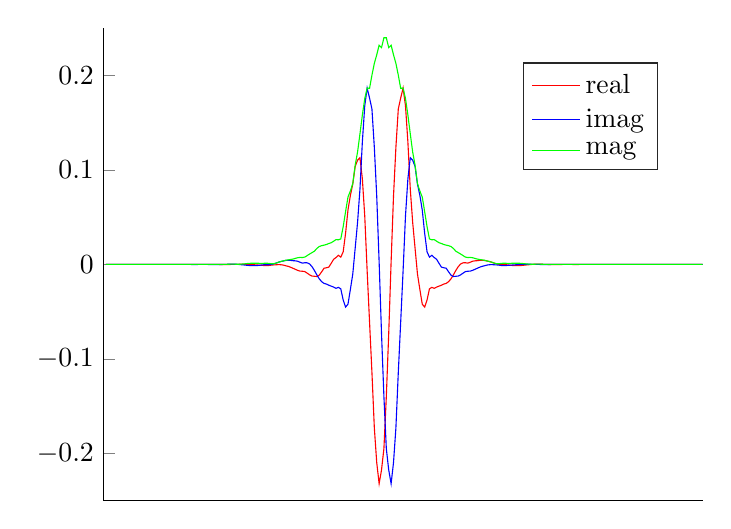
\begin{tikzpicture}

\begin{axis}[%
width=0.951\figurewidth,
height=\figureheight,
at={(0\figurewidth,0\figureheight)},
scale only axis,
xmin=0,
xmax=250,
xtick={\empty},
ymin=-0.25,
ymax=0.25,
axis background/.style={fill=white},
axis x line*=bottom,
axis y line*=left,
legend style={at={(0.7,0.7)},anchor=south west,legend cell align=left,align=left,draw=white!15!black}
]
\addplot [color=red,solid]
  table[row sep=crcr]{%
1	0\\
2	0\\
3	0\\
4	0\\
5	0\\
6	0\\
7	0\\
8	0\\
9	0\\
10	0\\
11	0\\
12	0\\
13	0\\
14	0\\
15	0\\
16	0\\
17	0\\
18	0\\
19	3.40598214094164e-12\\
20	0\\
21	-6.87793140105386e-11\\
22	-9.08261904251105e-11\\
23	4.62741351914918e-10\\
24	1.258882500922e-09\\
25	-3.90768164174049e-09\\
26	-4.94207941791755e-09\\
27	2.25257324923178e-08\\
28	4.47997487754667e-08\\
29	-3.72860948552819e-08\\
30	-7.72685694491778e-08\\
31	1.74091939763211e-07\\
32	3.20701693438365e-07\\
33	6.69906724002732e-08\\
34	-2.57334712035421e-07\\
35	-7.60438752193682e-07\\
36	-6.79175261479185e-07\\
37	3.85670908249705e-07\\
38	1.95760682064202e-06\\
39	2.70916484936271e-06\\
40	3.70985229264904e-06\\
41	5.60263903783335e-06\\
42	7.15200536225569e-06\\
43	9.42804407054984e-06\\
44	9.19816726897712e-06\\
45	4.09312377588624e-06\\
46	-2.18677142696421e-06\\
47	-7.78276608370347e-07\\
48	-2.49334758811333e-06\\
49	-1.24876312688003e-05\\
50	-2.40789294574741e-05\\
51	-5.00285382615212e-05\\
52	-5.19808121979403e-05\\
53	-8.56826227144868e-06\\
54	5.38557733758203e-05\\
55	9.09976831863687e-05\\
56	0.000118256932396166\\
57	0.000164847396440429\\
58	0.000172590561244501\\
59	0.000156541159523113\\
60	7.26324581485654e-05\\
61	-4.32251690266487e-05\\
62	-0.000209156467228341\\
63	-0.000355191843470207\\
64	-0.000528083903626197\\
65	-0.000723523151351148\\
66	-0.000904822353516488\\
67	-0.00117977622340421\\
68	-0.00127386800702199\\
69	-0.00107595626030387\\
70	-0.000731388490979029\\
71	-0.000492950213440953\\
72	-0.000355077529547522\\
73	-0.000176866907141536\\
74	-0.000304238537971187\\
75	-0.000669112865679403\\
76	-0.00137639751374934\\
77	-0.0019999871515232\\
78	-0.00288266647428663\\
79	-0.00399474325488351\\
80	-0.0051470769192401\\
81	-0.00623242432359724\\
82	-0.00706986688887293\\
83	-0.00719378257668194\\
84	-0.00758143497956961\\
85	-0.00925240669242568\\
86	-0.0110384455473666\\
87	-0.0122898662832043\\
88	-0.0125276118821436\\
89	-0.0127859505897159\\
90	-0.0113952391112889\\
91	-0.00784660452604257\\
92	-0.00401960851433002\\
93	-0.00350870901525763\\
94	-0.00282836192466074\\
95	0.00117836761234312\\
96	0.00541190932558586\\
97	0.00731202945632788\\
98	0.00961314726741875\\
99	0.00773250299419411\\
100	0.013341034228591\\
101	0.0329962818862013\\
102	0.0576135809313121\\
103	0.0730546535876305\\
104	0.084986015392322\\
105	0.103631123640744\\
106	0.110327196614011\\
107	0.112909993173503\\
108	0.0905813378752889\\
109	0.0513323912871931\\
110	-0.00674939368285724\\
111	-0.060713087095648\\
112	-0.114305418494503\\
113	-0.17300702433579\\
114	-0.209749288098405\\
115	-0.231992927271329\\
116	-0.217464614066301\\
117	-0.194784442562913\\
118	-0.140070485832163\\
119	-0.0733218645827401\\
120	0.00256331681737184\\
121	0.0722909879534431\\
122	0.123938750062336\\
123	0.164537100743611\\
124	0.1761522691017\\
125	0.186614921947609\\
126	0.16786851431561\\
127	0.129648576703118\\
128	0.0797149042875755\\
129	0.0445213447780424\\
130	0.0170433369608732\\
131	-0.0101767458153209\\
132	-0.0264788340863422\\
133	-0.0420467635360721\\
134	-0.0451140888775753\\
135	-0.0376649209952693\\
136	-0.0258341146252317\\
137	-0.0242550663754605\\
138	-0.0252504924158299\\
139	-0.0239210066309461\\
140	-0.0229612977291479\\
141	-0.0220048369351539\\
142	-0.0207817770698637\\
143	-0.0200383376462408\\
144	-0.0182129976759503\\
145	-0.0151705843558306\\
146	-0.0110133286799118\\
147	-0.00640572486704498\\
148	-0.00241914987168933\\
149	0.000501553892557113\\
150	0.00171502644229679\\
151	0.00182682703744143\\
152	0.00135819388712596\\
153	0.0023202015883891\\
154	0.00338143714657009\\
155	0.0038167928839548\\
156	0.00398922920965832\\
157	0.00435012390937784\\
158	0.00438744590069432\\
159	0.00420434222714658\\
160	0.00365909375507545\\
161	0.0031096699498426\\
162	0.00234243116660081\\
163	0.00139821952573963\\
164	0.000556075684303888\\
165	-5.51706115206466e-05\\
166	-0.000331691562229006\\
167	-0.000361308885120112\\
168	-0.00030880647995183\\
169	-0.000606048853947934\\
170	-0.000942240424391602\\
171	-0.00116480277977496\\
172	-0.00125325781851377\\
173	-0.00129181029001784\\
174	-0.00115716277061801\\
175	-0.000949777311562008\\
176	-0.000655071283282308\\
177	-0.000401238951280002\\
178	-0.000168066677392165\\
179	7.51939646498624e-05\\
180	0.000224400979048634\\
181	0.000325006343811925\\
182	0.00029951693903595\\
183	0.000193407642771761\\
184	5.23403692689068e-05\\
185	-7.08866952670796e-07\\
186	-1.49391620378925e-05\\
187	-3.63681852437294e-05\\
188	-3.66387543450729e-05\\
189	-4.31719371365099e-05\\
190	-3.68830397411496e-05\\
191	-1.45273881114298e-05\\
192	7.69634724727019e-06\\
193	1.40718734743013e-05\\
194	9.47996727945057e-06\\
195	1.08877455419357e-06\\
196	-8.37952554555356e-06\\
197	-9.54752048564336e-06\\
198	-6.25889587127397e-06\\
199	-2.89688757013566e-06\\
200	7.1722847502998e-07\\
201	1.69289428040498e-06\\
202	1.08252608403094e-06\\
203	5.10006804932853e-07\\
204	-3.13462849361191e-07\\
205	-3.54749535554903e-07\\
206	-1.07355897601877e-07\\
207	-3.86544340676565e-08\\
208	4.33594828396285e-08\\
209	5.64209933272261e-08\\
210	2.65249108795441e-08\\
211	1.4160405157173e-08\\
212	-9.40796883785182e-10\\
213	-2.76659516509318e-09\\
214	1.45966616149977e-09\\
215	3.51734339084897e-10\\
216	-1.27226347003132e-10\\
217	-8.49537384694854e-11\\
218	0\\
219	4.77098801261746e-12\\
220	0\\
221	0\\
222	0\\
223	0\\
224	0\\
225	0\\
226	0\\
227	0\\
228	0\\
229	0\\
230	0\\
231	0\\
232	0\\
233	0\\
234	0\\
235	0\\
236	0\\
237	0\\
238	0\\
239	0\\
240	0\\
241	0\\
242	0\\
243	0\\
244	0\\
245	0\\
246	0\\
247	0\\
248	0\\
249	0\\
250	0\\
};
\addlegendentry{real};

\addplot [color=blue,solid]
  table[row sep=crcr]{%
1	0\\
2	0\\
3	0\\
4	0\\
5	0\\
6	0\\
7	0\\
8	0\\
9	0\\
10	0\\
11	0\\
12	0\\
13	0\\
14	0\\
15	0\\
16	4.77098801261746e-12\\
17	0\\
18	-8.49537384694854e-11\\
19	-1.27226347003132e-10\\
20	3.51734339084897e-10\\
21	1.45966616149977e-09\\
22	-2.76659516509318e-09\\
23	-9.40796883785182e-10\\
24	1.4160405157173e-08\\
25	2.65249108795441e-08\\
26	5.64209933272261e-08\\
27	4.33594828396285e-08\\
28	-3.86544340676565e-08\\
29	-1.07355897601877e-07\\
30	-3.54749535554903e-07\\
31	-3.13462849361191e-07\\
32	5.10006804932853e-07\\
33	1.08252608403094e-06\\
34	1.69289428040498e-06\\
35	7.1722847502998e-07\\
36	-2.89688757013566e-06\\
37	-6.25889587127397e-06\\
38	-9.54752048564336e-06\\
39	-8.37952554555356e-06\\
40	1.08877455419357e-06\\
41	9.47996727945057e-06\\
42	1.40718734743013e-05\\
43	7.69634724727019e-06\\
44	-1.45273881114298e-05\\
45	-3.68830397411496e-05\\
46	-4.31719371365099e-05\\
47	-3.66387543450729e-05\\
48	-3.63681852437294e-05\\
49	-1.49391620378925e-05\\
50	-7.08866952670774e-07\\
51	5.23403692689068e-05\\
52	0.000193407642771761\\
53	0.00029951693903595\\
54	0.000325006343811925\\
55	0.000224400979048634\\
56	7.51939646498624e-05\\
57	-0.000168066677392165\\
58	-0.000401238951280002\\
59	-0.000655071283282308\\
60	-0.000949777311562008\\
61	-0.00115716277061801\\
62	-0.00129181029001784\\
63	-0.00125325781851377\\
64	-0.00116480277977496\\
65	-0.000942240424391602\\
66	-0.000606048853947934\\
67	-0.00030880647995183\\
68	-0.000361308885120112\\
69	-0.000331691562229006\\
70	-5.51706115206467e-05\\
71	0.000556075684303888\\
72	0.00139821952573963\\
73	0.00234243116660081\\
74	0.0031096699498426\\
75	0.00365909375507545\\
76	0.00420434222714658\\
77	0.00438744590069432\\
78	0.00435012390937784\\
79	0.00398922920965832\\
80	0.0038167928839548\\
81	0.00338143714657009\\
82	0.0023202015883891\\
83	0.00135819388712596\\
84	0.00182682703744143\\
85	0.0017150264422968\\
86	0.000501553892557114\\
87	-0.00241914987168932\\
88	-0.00640572486704498\\
89	-0.0110133286799118\\
90	-0.0151705843558306\\
91	-0.0182129976759503\\
92	-0.0200383376462408\\
93	-0.0207817770698637\\
94	-0.0220048369351539\\
95	-0.0229612977291479\\
96	-0.0239210066309461\\
97	-0.0252504924158299\\
98	-0.0242550663754605\\
99	-0.0258341146252317\\
100	-0.0376649209952693\\
101	-0.0451140888775753\\
102	-0.0420467635360721\\
103	-0.0264788340863422\\
104	-0.0101767458153209\\
105	0.0170433369608732\\
106	0.0445213447780424\\
107	0.0797149042875755\\
108	0.129648576703118\\
109	0.16786851431561\\
110	0.186614921947609\\
111	0.1761522691017\\
112	0.164537100743611\\
113	0.123938750062336\\
114	0.0722909879534431\\
115	0.00256331681737185\\
116	-0.0733218645827401\\
117	-0.140070485832163\\
118	-0.194784442562913\\
119	-0.217464614066301\\
120	-0.231992927271329\\
121	-0.209749288098405\\
122	-0.17300702433579\\
123	-0.114305418494503\\
124	-0.0607130870956479\\
125	-0.00674939368285723\\
126	0.0513323912871931\\
127	0.0905813378752889\\
128	0.112909993173503\\
129	0.110327196614011\\
130	0.103631123640744\\
131	0.0849860153923221\\
132	0.0730546535876306\\
133	0.0576135809313121\\
134	0.0329962818862013\\
135	0.013341034228591\\
136	0.00773250299419411\\
137	0.00961314726741875\\
138	0.00731202945632788\\
139	0.00541190932558586\\
140	0.00117836761234312\\
141	-0.00282836192466074\\
142	-0.00350870901525763\\
143	-0.00401960851433002\\
144	-0.00784660452604257\\
145	-0.0113952391112889\\
146	-0.0127859505897159\\
147	-0.0125276118821436\\
148	-0.0122898662832043\\
149	-0.0110384455473666\\
150	-0.00925240669242567\\
151	-0.00758143497956961\\
152	-0.00719378257668194\\
153	-0.00706986688887293\\
154	-0.00623242432359725\\
155	-0.00514707691924009\\
156	-0.00399474325488351\\
157	-0.00288266647428663\\
158	-0.0019999871515232\\
159	-0.00137639751374934\\
160	-0.000669112865679403\\
161	-0.000304238537971186\\
162	-0.000176866907141536\\
163	-0.000355077529547522\\
164	-0.000492950213440953\\
165	-0.000731388490979029\\
166	-0.00107595626030387\\
167	-0.00127386800702199\\
168	-0.00117977622340421\\
169	-0.000904822353516488\\
170	-0.000723523151351148\\
171	-0.000528083903626196\\
172	-0.000355191843470207\\
173	-0.000209156467228341\\
174	-4.32251690266487e-05\\
175	7.26324581485654e-05\\
176	0.000156541159523113\\
177	0.000172590561244501\\
178	0.000164847396440429\\
179	0.000118256932396166\\
180	9.09976831863687e-05\\
181	5.38557733758203e-05\\
182	-8.56826227144868e-06\\
183	-5.19808121979403e-05\\
184	-5.00285382615212e-05\\
185	-2.40789294574741e-05\\
186	-1.24876312688003e-05\\
187	-2.49334758811333e-06\\
188	-7.78276608370347e-07\\
189	-2.18677142696421e-06\\
190	4.09312377588625e-06\\
191	9.19816726897713e-06\\
192	9.42804407054984e-06\\
193	7.15200536225569e-06\\
194	5.60263903783335e-06\\
195	3.70985229264904e-06\\
196	2.70916484936271e-06\\
197	1.95760682064202e-06\\
198	3.85670908249705e-07\\
199	-6.79175261479185e-07\\
200	-7.60438752193682e-07\\
201	-2.57334712035421e-07\\
202	6.69906724002732e-08\\
203	3.20701693438365e-07\\
204	1.74091939763211e-07\\
205	-7.72685694491778e-08\\
206	-3.72860948552819e-08\\
207	4.47997487754667e-08\\
208	2.25257324923178e-08\\
209	-4.94207941791755e-09\\
210	-3.90768164174049e-09\\
211	1.258882500922e-09\\
212	4.62741351914918e-10\\
213	-9.08261904251105e-11\\
214	-6.87793140105386e-11\\
215	0\\
216	3.40598214094164e-12\\
217	0\\
218	0\\
219	0\\
220	0\\
221	0\\
222	0\\
223	0\\
224	0\\
225	0\\
226	0\\
227	0\\
228	0\\
229	0\\
230	0\\
231	0\\
232	0\\
233	0\\
234	0\\
235	0\\
236	0\\
237	0\\
238	0\\
239	0\\
240	0\\
241	0\\
242	0\\
243	0\\
244	0\\
245	0\\
246	0\\
247	0\\
248	0\\
249	0\\
250	0\\
};
\addlegendentry{imag};

\addplot [color=green,solid]
  table[row sep=crcr]{%
1	0\\
2	0\\
3	0\\
4	0\\
5	0\\
6	0\\
7	0\\
8	0\\
9	0\\
10	0\\
11	0\\
12	0\\
13	0\\
14	0\\
15	0\\
16	4.77098801261746e-12\\
17	0\\
18	8.49537384694854e-11\\
19	1.27271929686423e-10\\
20	3.51734339084897e-10\\
21	1.46128570001326e-09\\
22	2.76808565698103e-09\\
23	1.04844090692416e-09\\
24	1.42162533519356e-08\\
25	2.6811207973177e-08\\
26	5.66370253191664e-08\\
27	4.88615736180845e-08\\
28	5.91707931621314e-08\\
29	1.13646564485961e-07\\
30	3.6306702521868e-07\\
31	3.5856235360137e-07\\
32	6.02458726596314e-07\\
33	1.08459691719828e-06\\
34	1.7123411455216e-06\\
35	1.04531515880701e-06\\
36	2.97543889700524e-06\\
37	6.27076706447628e-06\\
38	9.74614651480286e-06\\
39	8.80658972302032e-06\\
40	3.86632048117235e-06\\
41	1.1011782045051e-05\\
42	1.57850816842511e-05\\
43	1.21705289920691e-05\\
44	1.71945132658123e-05\\
45	3.71094635206701e-05\\
46	4.32272845017189e-05\\
47	3.66470194482135e-05\\
48	3.64535551094453e-05\\
49	1.9470991168914e-05\\
50	2.40893614729532e-05\\
51	7.24042049593117e-05\\
52	0.00020027111903439\\
53	0.000299639469843039\\
54	0.000329438261050387\\
55	0.000242149494617008\\
56	0.000140138625580231\\
57	0.000235416805183551\\
58	0.000436783925820271\\
59	0.000673515791059104\\
60	0.000952550479258007\\
61	0.00115796981521183\\
62	0.00130863297114945\\
63	0.00130261905610722\\
64	0.0012789206875489\\
65	0.00118798264629529\\
66	0.00108903567654817\\
67	0.00121952178306504\\
68	0.00132411623726202\\
69	0.00112592236257258\\
70	0.00073346637353879\\
71	0.000743115118676452\\
72	0.00144260108628446\\
73	0.00234909890662455\\
74	0.00312451728830885\\
75	0.00371976869381013\\
76	0.0044239081905961\\
77	0.00482178702741808\\
78	0.00521855765790864\\
79	0.00564552241689185\\
80	0.00640783182766075\\
81	0.00709064384421969\\
82	0.007440857023028\\
83	0.0073208741551538\\
84	0.0077984263396001\\
85	0.00941001303398782\\
86	0.0110498342254224\\
87	0.0125256975598461\\
88	0.01407033654686\\
89	0.0168752464009988\\
90	0.0189736159996144\\
91	0.0198313511121225\\
92	0.0204375201096715\\
93	0.0210758937446378\\
94	0.0221858621585816\\
95	0.0229915146007476\\
96	0.024525564637458\\
97	0.026287889645464\\
98	0.0260906275367817\\
99	0.0269665177771404\\
100	0.0399578461365013\\
101	0.0558930732163425\\
102	0.0713249958400785\\
103	0.0777052833813811\\
104	0.0855931595844764\\
105	0.105023259908484\\
106	0.118971595154272\\
107	0.138214082220365\\
108	0.158157302115399\\
109	0.17554159761661\\
110	0.186736936380028\\
111	0.186321498637064\\
112	0.200345167693949\\
113	0.212819745880261\\
114	0.221857501106166\\
115	0.232007088031867\\
116	0.229492819488748\\
117	0.239918152847597\\
118	0.239918152847597\\
119	0.229492819488748\\
120	0.232007088031867\\
121	0.221857501106166\\
122	0.212819745880261\\
123	0.200345167693949\\
124	0.186321498637064\\
125	0.186736936380028\\
126	0.17554159761661\\
127	0.158157302115399\\
128	0.138214082220365\\
129	0.118971595154272\\
130	0.105023259908484\\
131	0.0855931595844765\\
132	0.0777052833813811\\
133	0.0713249958400785\\
134	0.0558930732163425\\
135	0.0399578461365013\\
136	0.0269665177771404\\
137	0.0260906275367817\\
138	0.026287889645464\\
139	0.024525564637458\\
140	0.0229915146007476\\
141	0.0221858621585816\\
142	0.0210758937446378\\
143	0.0204375201096715\\
144	0.0198313511121225\\
145	0.0189736159996144\\
146	0.0168752464009988\\
147	0.01407033654686\\
148	0.0125256975598461\\
149	0.0110498342254224\\
150	0.00941001303398781\\
151	0.0077984263396001\\
152	0.00732087415515381\\
153	0.007440857023028\\
154	0.0070906438442197\\
155	0.00640783182766075\\
156	0.00564552241689185\\
157	0.00521855765790864\\
158	0.00482178702741808\\
159	0.0044239081905961\\
160	0.00371976869381013\\
161	0.00312451728830885\\
162	0.00234909890662455\\
163	0.00144260108628446\\
164	0.000743115118676453\\
165	0.00073346637353879\\
166	0.00112592236257258\\
167	0.00132411623726202\\
168	0.00121952178306504\\
169	0.00108903567654817\\
170	0.00118798264629529\\
171	0.0012789206875489\\
172	0.00130261905610722\\
173	0.00130863297114945\\
174	0.00115796981521183\\
175	0.000952550479258007\\
176	0.000673515791059104\\
177	0.000436783925820271\\
178	0.000235416805183551\\
179	0.000140138625580231\\
180	0.000242149494617008\\
181	0.000329438261050387\\
182	0.000299639469843039\\
183	0.00020027111903439\\
184	7.24042049593117e-05\\
185	2.40893614729532e-05\\
186	1.9470991168914e-05\\
187	3.64535551094453e-05\\
188	3.66470194482135e-05\\
189	4.32272845017189e-05\\
190	3.71094635206701e-05\\
191	1.71945132658123e-05\\
192	1.21705289920691e-05\\
193	1.57850816842511e-05\\
194	1.1011782045051e-05\\
195	3.86632048117234e-06\\
196	8.80658972302032e-06\\
197	9.74614651480286e-06\\
198	6.27076706447628e-06\\
199	2.97543889700524e-06\\
200	1.04531515880701e-06\\
201	1.7123411455216e-06\\
202	1.08459691719828e-06\\
203	6.02458726596314e-07\\
204	3.5856235360137e-07\\
205	3.6306702521868e-07\\
206	1.13646564485961e-07\\
207	5.91707931621314e-08\\
208	4.88615736180845e-08\\
209	5.66370253191664e-08\\
210	2.6811207973177e-08\\
211	1.42162533519356e-08\\
212	1.04844090692416e-09\\
213	2.76808565698103e-09\\
214	1.46128570001326e-09\\
215	3.51734339084897e-10\\
216	1.27271929686423e-10\\
217	8.49537384694854e-11\\
218	0\\
219	4.77098801261746e-12\\
220	0\\
221	0\\
222	0\\
223	0\\
224	0\\
225	0\\
226	0\\
227	0\\
228	0\\
229	0\\
230	0\\
231	0\\
232	0\\
233	0\\
234	0\\
235	0\\
236	0\\
237	0\\
238	0\\
239	0\\
240	0\\
241	0\\
242	0\\
243	0\\
244	0\\
245	0\\
246	0\\
247	0\\
248	0\\
249	0\\
250	0\\
};
\addlegendentry{mag};

\end{axis}
\end{tikzpicture}% 
      \caption{Real, Imaginary and Modulus of complex wavelet convolved with
               an impulse.}
      \label{fig:pulse_response}
    \end{center}
  \end{figure}
  

  % A tikz diagram to draw what the operator looks like so far
  %\input{tikz/invariant}

  The modulus can be made fully invariant by integrating, i.e.,:
  $$\int F x(\bmu{u})d\bmu{u}= \int | x \ast \psi_{\lambda}(\bmu{u})| d\bmu{u}$$
  is translation invariant. 
  Total invariance to shifts means integrating over the entire function, which
  may not be ideal as it loses a significant amount of information in doing this. Instead
  \citeauthor{bruna_invariant_2013} define scales $2^J$, over which their operator
  is invariant to shifts. Now instead of integrating, the output $\|x \ast \psi_{\lambda}\|$ is
  convolved with an averaging window, or conveniently, the scaling function for
  the chosen wavelet:
  $$\phi_{2^J}(\bmu{u}) = 2^{-2J}\phi(2^{-J}\bmu{u})$$

  Even still, this averaging means that a lot of information is lost from the
  first layer outputs ($\|x \ast \psi_{\lambda}\|$).
  \citeauthor{bruna_invariant_2013} combat this by also convolving the output
  with wavelets that cover the rest of the frequency space, giving  
  $$U[p]x = U[\lambda_2]U[\lambda_1]x = \| | x \ast \psi_{\lambda_1}| 
    \ast \psi_{\lambda_2} \|$$
  The choice of wavelet functions $\lambda_{1}$ and $\lambda_{2}$ is combined
  into a path variable, $p = (\lambda_1, \lambda_2, \ldots \lambda{m})$.

  Local invariants can be again computed by convolving this with another scaling
  function $\phi$. The result is now a multiscale scattering transform, with
  coefficients:
  $$ S[p]x = U[p]x \ast \phi_{2^J}(\bmu{u}) $$
  A graphical representation of this is shown in
  \autoref{fig:scatternet_mallat}.

  \begin{figure}
    \centering
      \includegraphics[width=\textwidth]{images/scatternet_diagram.png}
      \caption[Translation Invariant Scatternet Layout]
              {The translation invariant Scattering Transform. Scattering outputs
               are the leftward pointing arrows $S[p]x$, and the intermediate 
               coefficients $U[p]x$ are the centre nodes of the tree. Taken
               from \citep{bruna_invariant_2013}.}
      \label{fig:scatternet_mallat}
  \end{figure}

  % \begin{eqnarray*}
  % \bm{lambda} &=& (j, \theta)
  % % Scattering transform equation
  % \begin{eqnarray*}
  % \Phi x & = & \{S[\bmu{p}]x(\bmu{u}) | \bmu{p} = (\bmu{\lambda_{1}},
  % \bmu{\lambda_{2}}, \ldots \bmu{\lambda_{m}})

\section{Rotation and Translation Invariant Scatternets}
  Mallat's group refined their Scatternet architecture by expanding their list
  of invariants to also include rotation. They also experimented with adding
  scale invariance in \citep{sifre_rotation_2013}, but it was limited to only
  averaging over scale once, and they were no longer using
  it in \citep{oyallon_deep_2015}, so for brevity we omit it. 
  
  This work was done by two authors, each tackling different
  challenges. The first is texture analysis with Sifre in
  \citep{sifre_combined_2012, sifre_rotation_2013, sifre_rigid-motion_2014,
  sifre_rigid-motion_2014-1}, and the second is image classification with
  Oyallon in \citep{oyallon_generic_2013, oyallon_deep_2015}. In this section,
  we outline the properties and structure of this extended Scatternet.

\subsection{An Important note on Joint vs. Separable Invariants}
  When building multiple invariants, some thought must be given as to how to
  combine them --- separably or jointly? Let us call the group of operations we
  want to be invariant to $G$, with $g \in G$ a single realization from this
  group --- in this case, $G$ is the group of affine transformations. We want
  our operator $\Phi$ to be invariant to all  $g \in G$, i.e.,\ $\Phi(gx)
  = \Phi(x)$. Building separable invariants would mean representing the group
  as $G=G_2G_1$ (an assumption of the group, not of our model), and building
  $\Phi = \Phi_2 \Phi_1$, where $\Phi_1$ is invariant to members of $G_1$ and
  covariant to members of $G_2$, and $\Phi_2$ is invariant to members of $G_2$.
  I.e.,\
  \begin{equation}
    \Phi_2(\Phi_1(g_1g_2x)) = \Phi_2(g_2\Phi_1(x)) = \Phi_2(\Phi_1(x))
  \end{equation}
  An example of this would be in the group $G$ of 2D translations, building
  horizontal invariance first, then building vertical invariance second.
  \Bruna\ warn about this approach, however, as it cannot capture the action
  of $G_2$ relative to $G_1$. In the case of veritcal and horizontal
  translations, for example, it would not be able to distinguish if the
  patterns had moved apart as well as being shifted, whereas a joint
  horizontal and vertical translation invariant would be able to distinguish
  these two cases.

  % \begin{figure}[t!]
    % \centering
  % %    \captionsetup[subfigure]{width=0.3\textwdith}
      % \subfloat[]{\includegraphics[width=0.3\textwidth]{scripts/separable_invariance_1.png}
                  % \label{fig:joint_pattern1}}
  % %    \quad   
      % \subfloat[]{\includegraphics[width=0.3\textwidth]{scripts/separable_invariance_2.png}
                  % \label{fig:joint_pattern2}}
  % %    \quad
      % \subfloat[]{\includegraphics[width=0.3\textwidth]{scripts/separable_invariance_3.png}
                  % \label{fig:joint_pattern3}}
      % \caption[Patterns illustrating the difference between joint and separable invariants]
              % {Patterns illustrating the difference between joint and separable
              % invariants. \subref{fig:joint_pattern1} the reference pattern.
              % \subref{fig:joint_pattern2} pattern shifted horizontally and
              % vertically.  \subref{fig:joint_pattern3} pattern shifted apart.
              % A joint invariant would be able to distinguish
              % between~\subref{fig:joint_pattern2}
              % and~\subref{fig:joint_pattern3}, but a separable invariant would
              % not.}
      % \label{fig:joint_pattern}
  % \end{figure}

  In this vein, \Bruna\ suggest that in the case of rotation and translation
  invariance, a joint invariant should be used, building on the work in
  \citep{citti_cortical_2006, boscain_anthropomorphic_2010,
  sgallari_scale_2007}. 

  % \begin{figure}
    % \centering
      % \includegraphics[width=7cm]{images/scatternet_roto_scale_block.png}
      % \caption{Roto-Translation and Scale Invariant Scatternet block diagram. The
               % log operation between roto-translation and scale invariances is used to
               % linearize the power law of the Scatternet coefficient energies across 
               % scales. Taken from \citep{sifre_rotation_2013}.}
      % \label{fig:roto_scat_block}
  % \end{figure}

\subsection{Defining the Properties}
  A translation $g = (v, \theta)$ of the roto-translation group $G_{rt}$ acting on
  $\bmu{u} \in \mathbb{R}^2$ combines translation by $v$ and rotation by
  $R_{\theta}$ as:
  \begin{equation}
    g\bmu{u} = v + R_{\theta}\bmu{u}
  \end{equation}
  The product of two successive roto-translations $h=(v',
  \theta ')$ and $g = (v, \theta) $is:
  \begin{equation}
    gh = (v + R_{\theta}v', \theta + \theta')
  \end{equation}
  In much the similar approach to the simple translation invariant Scatternet defined
  above, \Bruna\ calculate successive layers of signal coefficients $U[p]x$ that
  are covariant to the actions of all $g \in G_{rt}$ --- i.e.,\ 
  \begin{equation}
    U[p](gx) = gU[p]x
  \end{equation}
  Creating invariants of order $m = \mathrm{length}(p)
  = \mathrm{length}([\lambda_1, \lambda_2, \ldots, \lambda_m])$ is then done by
  averaging $hU[p]x$ for all h in $G_{rt}$
  \begin{equation}
    S[p]x(g) = \sum_{h \in G_{rt}} hU[p]x \Phi_J(h^{-1}g)
  \end{equation}
  This convolution averages $hU[p]x$ over all rotation angles in a spatial
  neighbourhood of $\bmu{u}$ of size proportional to $2^J$.

\subsection{The Operator}
\subsubsection{Roto-Translation Invariance}
  Although we want to have a joint invariant for rotations and translations,
  this can be done with a cascade of wavelet transforms --- so long as the
  final averaging operation is done over both rotation and translation. \Sifre\
  do just this, building a 3 layer scattering transform, the first layer of
  which is exactly identical to the previous translation scattering transform,
  i.e.,\
  \begin{equation}
    \tilde{W}_1 x = \left( x \ast \phi_J, \{|x \ast \psi_{\theta, j}|\} \right)
      = (S_0x, U_1x)
  \end{equation}
  The second and third layers are, however, new. The invariant part of $U_1$ is
  computed with an averaging over spatial and angle variables. \emph{This
  averaging  is implemented at fixed scales j} (see our note earlier about
  choosing separable scale invariance). For an action $g = (v, \theta)$, the
  averaging kernel is defined as:
  \begin{equation}
    \Phi_J(g) =  \bar{\phi}(\theta) \ast \phi_J(u)
  \end{equation}
  Where $\phi_J(u)$ is a kernel that averages each $U_1x$ over scale $2^J$,
  and $ \bar{\phi}(\theta= (2\pi)^{-1})$ averages the result of that average over all angles.

  To clarify, we look at an example architecture with $J=2$ scales and $L=4$
  orientations. The output of the first layer $U_1x$ would be a set of
  coefficients:
  \begin{equation}
    U_1x = \left\{ |x \ast \psi_{j, \theta} | \, \middle| \, j=\{0,1\}, \,
    \theta=k\pi/4, \, k= \{0,1,2,3\} ,\right\}
  \end{equation}
  i.e.,\ there would be 4 high frequency coefficients, which were created with
  wavelets centred at $|\bm{\omega}| = 3\pi/4$, and 4 medium frequency components
  created with wavelets centred at $|\bm{\omega}| = 3\pi/8$. Each of these 8 will
  be averaged across the entire image, then each pair of 4 will be averaged
  across all 4 rotations, leaving 2 invariants.

  To recover the information lost from averaging, \Sifre\ also convolve $U_1x$
  with corresponding rotation and scale wavelets to pass on the high frequency
  information. These roto-translation wavelets, while joint, can also be computed
  with the cascade of separable wavelets. It may be helpful to consider the
  spatial variable $\bmu{u}$ as single dimensional, and consider the rotation
  variable $\theta$ as a second dimension. The above equation calculated the low-low
  frequency component of these two variables, the remaining components are the
  low-high, high-low, and high-high. 

  We define the low frequency spatial scaling functions $\phi_J(u)$\footnote{we
  temporarily drop the boldface from the spatial parameter u to make it clearer
  it can be considered as single dimensional}, the spatial wavelets
  $\psi_{\theta, j}(u)$, the rotation scaling function $\bar{\phi}(\theta)$
  (which is just the constant $(2\pi)^{-1}$, but we write out in generic form
  nonetheless), and the rotation wavelet $\bar{\psi}_k(\theta)$, which is
  a $2\pi$ periodic wavelet.

  Then, the remaining low-high, high-low, and high-high information is:
  \begin{eqnarray}
    \Psi_{0, J, k_2}(u, \theta) & = & \phi_J(u) \ast \bar{\psi}_{k_2}(\theta) \\
    \Psi_{\theta_2, j_2, } (u, \theta) & = & \psi_{\theta_2, j_2}(u) \ast
      \bar{\phi}(\theta) \\
    \Psi_{\theta_2, j_2, k_2}(u, \theta) & = & \psi_{\theta_2, j_2}(u) \ast
      \bar{\psi}_{k_2}(\theta)
  \end{eqnarray}
  The k parameter is newly introduced here, and it represents the number of
  scales the rotation wavelet has (a typical value used by \Sifre\ was $K=3$).
  We call this combined operator $\Psi_{\theta_m, j_m, k_m}$. See
  \autoref{fig:srs_3d} for what this looks like.

  \begin{figure}
    \centering
      \includegraphics[width=9cm]{images/scatternet_roto_scale_3dwavelet.png}
      \caption[Three dimensional convolution with roto-scale wavelet]
              {Three dimensional convolution with  $\Psi_{\theta_m, j_m,
              k_m}(u_1, u_2, \theta)$ factorised into a two dimensional convolution with
              $\psi_{\theta_m, j_m}(u_1, u_2)$ and a one dimensional convolution with
              $\psi_{k_m}(\theta)$. Colours represent the amplitude of the 3D
              wavelet. Image taken from \citep{sifre_rotation_2013}.}
      \label{fig:srs_3d}
  \end{figure}

  The wavelet-modulus operator then is:
  \begin{equation}
    \tilde{W}_m Y = \left( Y \ast \Phi_J(g), |Y \ast \Psi_{\theta_m, j_m, k_m}
      (g)| \right)
  \end{equation}
  for $m\ge 2$ and the final third order roto-translation Scatternet is:
  \begin{equation}
    Sx = (x\ast \phi_J(\bmu{u}), U_1x \ast \Phi_J(p_1), U_2x \ast \Phi_J(p_2))
    \label{eq:roto_shift}
  \end{equation}
  with $p_1 = (\bmu{u}, \theta_1, j_1)$ and $p_2=(\bmu{u}, \theta_1, j_1,
  \theta_2, j_2, k_2)$.


